\chapter{Implementation Details}
\label{developed-work}
In this Chapter we describe the implementation details of the project and employed technologies. In Section~\ref{sec:DataBaseModel} we start by detailing the Service and Log databases. Section~\ref{sec:dal} approaches the Data Access Layer, and how it interacts with the database. In Section~\ref{sec:RestAPIImplementation} we introduce the implementation aspects of the REST API and its communication with the DAL. Section~\ref{sec:recommenderService} describes the technical aspects of the recommender system. Then in Section~\ref{sec:iosApplication} we detail the development of the mobile application, followed by Section~\ref{subsec:pushNotificationIntro} with information regarding the implemented Apple Push Notification Service Provider. Section~\ref{sec:mobileApp} is dedicated to the developments of the Web application. We finish the current Chapter with Section~\ref{sec:additionalImplementation}, describing additional developments that were made.

\section{Database Model}
\label{sec:DataBaseModel}
In this Section, we introduce some implementation details of the databases, which were developed using the MySQL technology.

\subsection{Service Database}
\label{sec:ServiceDataBaseModel}
The service database is designed to store and access, in a structured way, information regarding the touristic locations, users data, visited locations, among other fields. The~\gls{er} model for the Service Database is presented in Appendix~\ref{sec:ServiceDatabase}.\\
\\
One of the objectives of the project is to support multilanguage. In order to provide this kind of support, some preparations were made at the database level. The \verb"Locale" table was introduced, which is responsible for controlling the language of the different items. To demonstrate the localization functionality, the project was developed supporting two different languages: Portuguese [PT] and English [EN]. We use the language identifier as defined by the ISO 639-1 standard~\cite{rfcLanguageCode}.\\
\\
In order to provide the location with the descriptive information regarding weather conditions and time of visit, a standard approach would be to create a separate table for the attribute in cause and to have a many-to-many relationship between this table and the \verb"Location" table (each attribute would generate two additional tables). By using the proposed solution, the complexity of the database model is minimized because the information is organized in a way such that the number of existing tables is reduced, which minimizes the need for the additional \emph{join} operations during the query execution. A mask of bits is used to characterize some attributes of the point of interest. Table~\ref{tab:bitMaskWeatherColumns} and Table~\ref{tab:bitTimeSeasonMask} describe the proposed solutions to characterize the following components of the location:
\begin{itemize}
\item \verb"visitWeatherMask" - represents the possible values for the weather condition.
\item \verb"visitTimeMask" - describes the time of day for the visit.
\end{itemize}
%%%%%%%
\begin{center}
\begin{table}
	\centering
    \caption{Bitmask for the \textbf{visitWeatherMask} column.}
    \label{tab:bitMaskWeatherColumns}
   \begin{tabular}{| >{\centering\arraybackslash}m{2.6cm} | >{\centering\arraybackslash}m{2.6cm} |>{\centering\arraybackslash}m{2.6cm} |>{\centering\arraybackslash}m{2.6cm} |>{\centering\arraybackslash}m{2.6cm} |>{\centering\arraybackslash}m{2.6cm} |>{\centering\arraybackslash}m{2.6cm} |>{\centering\arraybackslash}m{2.6cm} |}
    \hline
	Sun & Rain and Clouds & Snow
    \\ \hline    
	0x1 & 0x2 & 0x4
    \\ \hline
    \end{tabular}
    \end{table}
\end{center}
%%%%%%%%%%
\begin{center}
\begin{table}
	\centering
    \caption{Bitmask for the \textbf{visitTimeMask} column.}
    \label{tab:bitTimeSeasonMask}
   \begin{tabular}{| >{\centering\arraybackslash}m{3.9cm} | >{\centering\arraybackslash}m{3.9cm} |>{\centering\arraybackslash}m{3.9cm} | >{\centering\arraybackslash}m{3.9cm} |}
    \hline
	Day & Night\\ \hline    
	0x1 & 0x2 \\ \hline
    \end{tabular}
    \end{table}
\end{center}
%%%%%%%%%%
A similar approach is used to define the \verb"profileMask" attribute for the \verb"User" table which represents the user's role in the system. Table~\ref{tab:bitProfileMask} shows the possible mask values for this attribute.
\begin{center}
\begin{table}
	\centering
    \caption{Bitmask for the \textbf{profileMask} column.}
    \label{tab:bitProfileMask}
   \begin{tabular}{| >{\centering\arraybackslash}m{3.9cm} | >{\centering\arraybackslash}m{3.9cm} |>{\centering\arraybackslash}m{3.9cm} | >{\centering\arraybackslash}m{3.9cm} |}
    \hline
	Admin & Standard \\ \hline    
	0x1 & 0x2 \\ \hline
    \end{tabular}
    \end{table}
\end{center}
%%%%%%%%%%
Each role purpose is described below:
\begin{itemize}
\item \verb"Admin" - User with the highest privilege access, being allowed to consult and edit any information regarding the point of interest.
\item \verb"Standard" - Has access to consult information regarding the touristic location.
%\item \verb"Contributor" - Can access points of interest with the \verb"Active" or \verb"Testdrive" state.
\end{itemize}
These bit mask attributes are stored as integer values, where each power of two value represents different information that can be merged with other values through bitwise operations. An efficient approach is possible due to the well-defined domain values. Even if there is a need to insert new values, those can be easily added to the existing set. Assuming that the augmented set is composed by $n$ elements, the newly added value will occupy the index $2^n$, with $n~\epsilon~\{0;~31\}$ allowing a total of 32 different values.\\
\\
Two different scripts were created for the database population. Each one performs insertions in the following tables, based on its \verb"Locale" value:\\
\\
\begin{itemize}
   \item \verb"Locale" - Representation of the English and Portuguese locales.
   \item \verb"Country" - A set of 249 countries with English description and other 249 with Portuguese description.
   \item \verb"Status" - Allowed values for the location attractions filled in English and Portuguese.
   \item \verb"Attraction" - Allowed values to describe attractions of the location in English and Portuguese.
   \item \verb"SocialService" - Contains information regarding the social services that are supported by the system, currently used for authentication purposes.
\end{itemize}
The GuideMe service supports the social interaction by allowing users to follow and to be followed. The Follower table was created in order to represent this relationship; its definition is presented in Appendix~\ref{sec:ServiceDatabase}.
%%%%%%%
%%%%%%%
\subsection{Log Database}
\label{sec:LogDataBaseModel}
The log database is used to track the different kind of events that may occur in the system, such as errors, warnings, and other informative messages. The~\gls{er} model for the Log database is presented in Appendix~\ref{sec:AttachmentsLogDatabase}.
\\
The choice of performing the log into the database instead of a different method consists in providing a more interactive way to access the log data. Using this approach, it becomes easier to implement client applications with friendly user interfaces that can access, filter, and manipulate log information.\\
\\
The logged information can be crucial to detect bugs. We have implemented the alternative logger solution using the Log4j~\cite{apacheLog4j} library, which ensures persistence of this information when the logging to the database fails due to some disruption causes. Each system component can optionally specify the configuration file, which is used to configure the logger properties as well as the destination of the file that should be used for logging. By default, the configuration file is located under the root directory of the corresponding project and is named as \emph{LocalLocagger.properties}.

%%%%%%%%%%%%%%%%%%%%%%%%%%%%%%%%%%%%%%%%%%%%%%%%%%%%%%%%%%%%
\section{Data Access Layer}
\label{sec:dal}
In this Section, we describe the key aspects of the \gls{dal} implementation, which was written in Java using the Hibernate framework.

\subsection{Implementation Details}
\label{subsec:logDbDAL}
Some implementation details of the \gls{dal} for both the Service and Log databases are described in this Subsection. In order to not compromise the \gls{dal} usage with the Hibernate framework, a \gls{dao}~\cite{dao} pattern is used to encapsulate the access to the data with an interface. The layers above \gls{dal} are independent from the Hibernate framework, allowing this to be easily replaced, if needed. Different projects were currently configured in the Eclipse~\cite{eclipse}~\gls{ide}; the aim of each one of them is as follows:
\begin{itemize}
\item \verb"DALCommon" - contains a set of classes that are common between the \verb"GuideMeLogDAL" and \verb"GuideMeServiceDAL". It offers a generic implementation for the Entity Objects\footnote{Entity Objects - are the components that encapsulate the data model. Any instance is mapped into a single object in the data source.}, \gls{dao} interfaces, as well as the exception hierarchy.
\item \verb"GuideMeLogDAL" - represents the implementation of the \gls{dal} that provides methods to manipulate the Log database. It allows to log events that occur in different applications. Contains the test cases that perform unitary testing against the \gls{dao} implementation.
\item \verb"GuideMeServiceDAL" - contains the implementation of the \gls{dal} for the service database. Provides different methods to query the data that represent the core information of the service. Implements unitary tests for every written operation.
\end{itemize}
\verb"DALCommon" defines a generic set of classes and interfaces that generalise the implementation and access to specific database operations. Figure~\ref{fig:dalUMLDiagrama} shows the~\gls{uml}~\cite{umlLanguage} diagram with main components of the DAL. 
\\
\begin{figure}[h!]
 \centering
   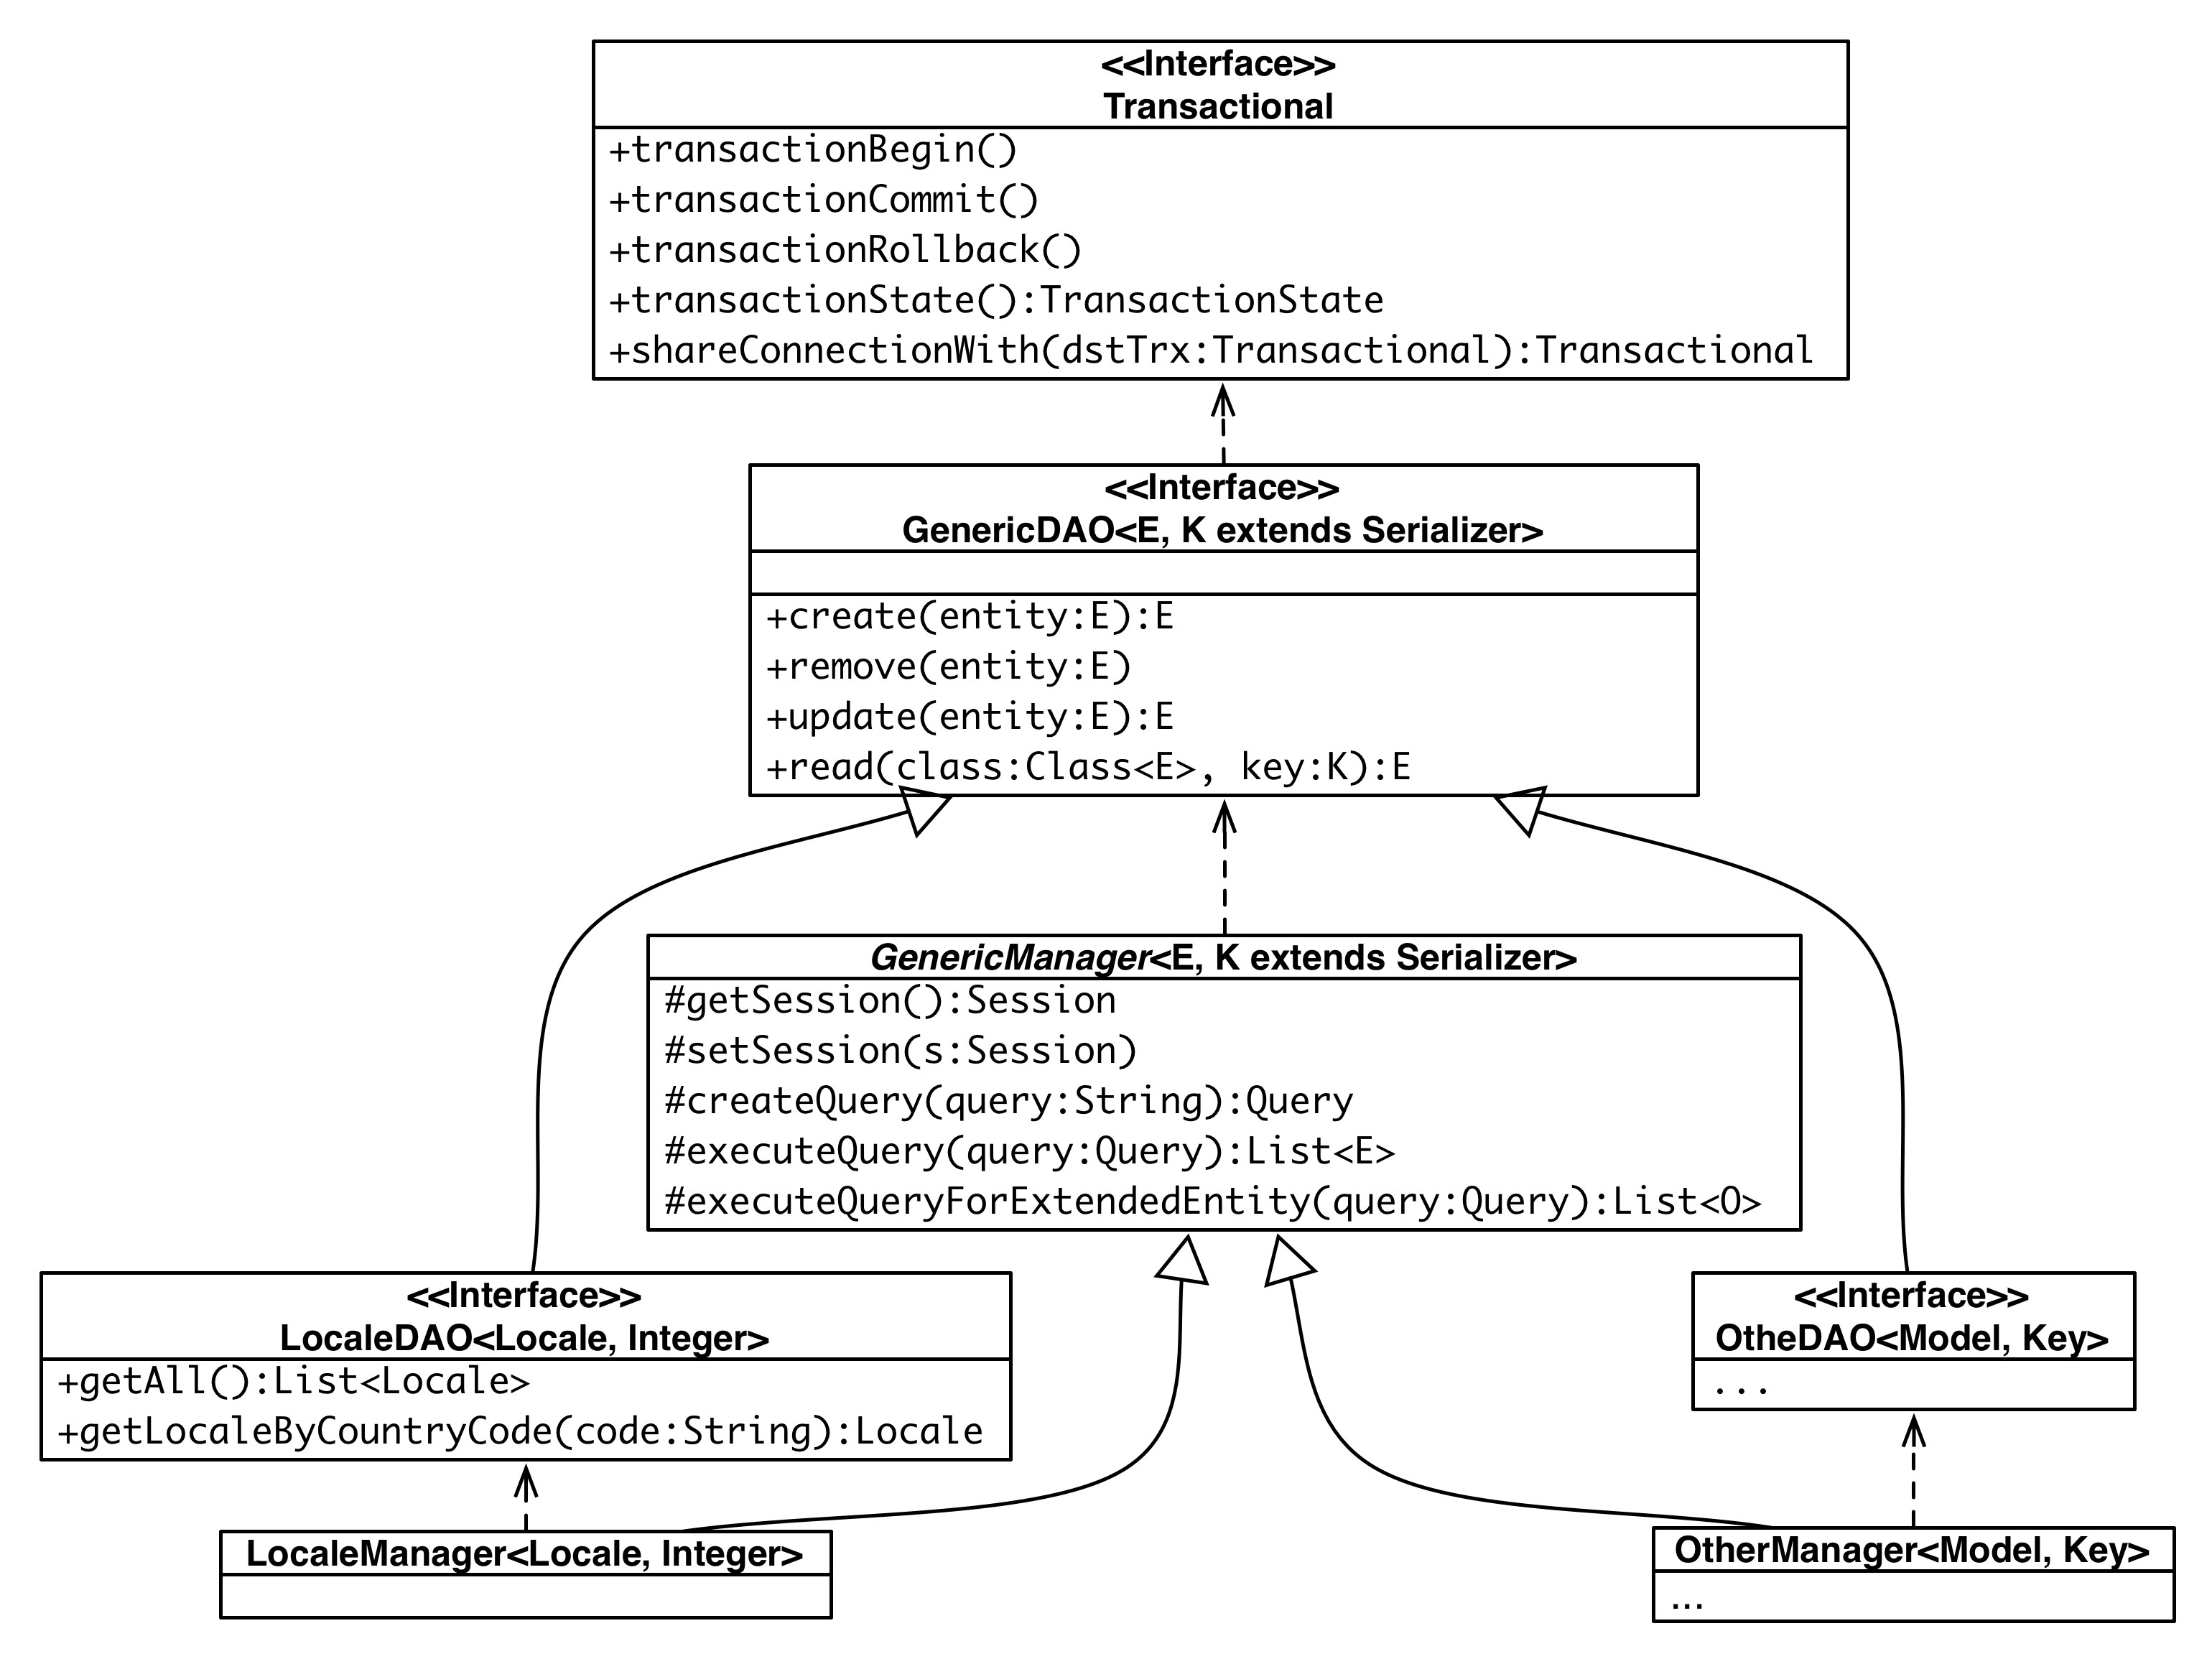
\includegraphics[width=13.2 cm]{./images/umls/uml_diagram_dal.jpg}
   \caption{UML diagram of the DAL core classes.}
   \label{fig:dalUMLDiagrama}
\end{figure}
\\
On top, we have the \verb"Transactional" interface which describes the contract for the manipulation of the transaction. Then the \verb"GenericDAO" describing the CRUD (Create, Read, Update and Delete) operations. The \verb"GenericManager" class implements both interfaces, \verb"Transactional" and \verb"GenericDAO", and it also offers additional helper methods that simplify the implementation of the operations for accessing data.\\
\\
The \verb"GenericDAO" interface and the \verb"GenericManager" class are implemented by each hibernate entity that requires to be accessed within a query. In the concrete \verb"DAO" interface, we describe specific methods that query the database to obtain data and the concrete \verb"Manager" class provides an implementation for those methods as well as for the CRUD operations inherited from the \verb"GenericManager". The specific operations use the~\gls{hql} which is similar to SQL. The Hibernate framework is then responsible for converting the~\gls{hql} into the corresponding SQL code.\\
\\
The service database and log database \gls{dal} uses the structure illustrated in Figure~\ref{fig:dalUMLDiagrama} and both follow the same implementation flow, previously described.
%%%%%%%
%%%%%%%
\subsection{Hibernate Framework Configuration}
\label{subsubsec:hfc}
In this Subsection we describe the configuration aspects of the Hibernate framework along with the additional functionalities that were implemented. We also detail some obstacles that have emerged during the development of the DAL.\\
\\
The Hibernate framework is configured with the \emph{hibernate.cfg.xml} file which contains the information such as the database name, location, user name, password, among others fields. The configuration file also includes information regarding the entity mappings which are defined as a list of references to \gls{hbm} files. The Hibernate tool was installed for the Eclipse IDE, allowing to reverse engineer entities from the database. The auto-generated entity represents the Java object with the associated mapping \gls{hbm} file which describes the attributes and relationship to other entities.\\
\\
Another required configuration of the Hibernate framework is the dialect, which is responsible for generating appropriate SQL for the chosen database. A suitable dialect for our MySQL database is the \verb"MySQL5InnoDBDialect". We had a need to extend it in order to add the mapping for the bitwise operations, since those are not included in the original dialect and cannot be used in \gls{hql}. When the Hibernate framework is initialized, our custom dialect performs registry of the two custom functions (\verb"bitwise_and" and \verb"bitwise_or") that can be used in a \gls{hql} query in order to be correctly converted into corresponding SQL query. The Code Listing~\ref{cod:sqlVShql} shows the usage example for the \gls{hql} with custom defined binary operation which is then mapped to SQL.

\lstset{language=SQL} 
\begin{lstlisting}[frame=single,caption={SQL mapped from HQL.}, label={cod:sqlVShql}, frame=bt]
/* HQL */
SELECT e FROM Entity e WHERE bitwise_and(e.binary1, :someVal) = :someVal
/* SQL */
SELECT e.* FROM entity WHERE e.binary1 & ? = ?
\end{lstlisting}
%%%%%%%
%%%%%%%
\subsection{Difficulties Found in the Implementation}
\label{subsubsec:odi}
Some difficulties were found during the implementation of the DAL, more specifically on the data mapping of the \verb"Localized_Location" table. The first approach consisted in making the field \verb"locale_id" as part of the composite~\gls{pk} and also as the~\gls{fk} for the \verb"city" and \verb"attraction" tables. The~\gls{er} model was valid and successfully generated, but during the creation of the new \verb"Localized_Location" record through the Hibernate framework, the \gls{fk} relationship for the \verb"city" and \verb"attraction" were not included in the generated SQL INSERT statement. This behaviour caused the insertion statement to fail, since \verb"attraction_id" and \verb"city_id" could not be \verb"null".\\
\\
A suitable solution was found for this problem, which consisted in replicating the \verb"locale_id" attribute. The following set of fields were created \{\verb"location_locale_id", \verb"city_locale_id", \verb"attraction_locale_id"\} to replace the original \verb"locale_id".
The implementation of the~\gls{dal} guaranties that has the three fields have always the same value for the specific record.\\
\\
Another problem has emerged when it became necessary to specify different databases in the configuration file. When the hibernate models are generated using the Hibernate Reverse Engineering tool, one of the attributes in the created files is the \emph{catalog} which points to the database used during the code generation process. This binds the model to that database, which is not what we need. However, when the \emph{catalog} attribute is not indicated, the hibernate engine automatically uses the database defined in the configuration file.\\
\\
To circumvent this binding problem, the solution consisted in the creating the Ant~\cite{antTask} task that removes the \emph{catalog} attribute, for each hibernate model file. After generating the hibernate model, it is required to execute the defined Ant task in order to re-process the HBM files.

%%%%%%%%%%%%%%%%%%%%%%%%%%%%%%%%%%%%%%%%%%%%%%%%%%%%%%%%%%%%
\section{REST API}
\label{sec:RestAPIImplementation}
This Section describes different aspects of the implemented \gls{rest}~\gls{api}, and the technologies and methodologies used to design the API.\\
\\
The \gls{rest}~\gls{api} was implemented using the Play Framework. It integrates the components and API required for web application development. The framework is based on a lightweight, stateless, web-friendly architecture that optimizes the resource consumption for scalable applications~\cite{playPerformance}.\\
\\
Our API provides a set of endpoints whose purpose is to obtain data through DAL and serialize the response into \gls{json} format. Every response is composed with header and body. The header contains the information that allows to identify if the request is successfully executed or not. An example of this scenario is illustrated on Code Listing~\ref{cod:guideMeAPIResultEx}. When the header contains the information regarding an error, the body is populated with the null value. The detailed version of the API documentation can be accessed through \verb"Settings/API Documentation" on the Web application.\\
\\
\begin{lstlisting}[language=json,firstnumber=1,caption={Example of the success and error headers.},label={cod:guideMeAPIResultEx}]
/* Success */
{
    "header": {
        "operationSucceeded": true,
        "sessionState": "SessionStateValid" or "SessionStateNotRequired"
    },
    "body": ...
}

/* On error */
{
    "header": {
        "errorMessage": "Length of the locale identifier argument should be exactly 2",
        "operationSucceeded": false,
        "validArguments": false,
        "sessionState": "SessionStateInvalid",
        "friendlyErrorMessage": "Error communicating with the server. Please try again later."
    },
    "body": null
}
\end{lstlisting}
%%%%%%%
%%%%%%%
\subsection{Internationalization Support}
\label{sec:apiInternationalization}
Internationalization is the technique for organizing localized resources so that an application can select the user-preferred set of resources at runtime. Localization is the translation of text displayed by an application. The importance of supporting multiple languages consists in reaching the maximum number of users, specifically in tourist guide applications where users of the application are from different countries. Currently, the API supports English and Portuguese languages, and it is possible to add other languages.\\
\\
Every endpoint receives the \verb"localeName" argument which should have the ISO 639-1 format and sends the response in the corresponding language. The English language is assumed by default when the \verb"localeName" argument is not specified or refers to the unsupported language.\\
\\
When an error occurs during the request, some properties of the header information are populated with the localized information regarding the error in cause, namely the \emph{errorMessage} and \emph{friendlyErrorMessage} properties. These messages are defined as a property list in the \verb"conf/messages.pt" and \verb"conf/messages.en" files. The Play framework offers an easy way to access the localized i18n~\cite{i18nOrigin} properties, as it is shown in Code Listing~\ref{cod:i18nDefinAndUse}.
\newpage
\begin{lstlisting}[language=java,caption={An example of the i18n definition and usage.},label={cod:i18nDefinAndUse}, frame=bt]
Message.UserName=Nome Completo    # messages.pt
Message.UserName=Full Name        # messages.en
------------------------------
// Depending on the current language, the framework will obtain 
// the localized value for the  Message.UserName key
String example = Messages.get("Message.UserName") + ":" + user.getName();
\end{lstlisting}
%%%%%%%
%%%%%%%
\subsection{Implementation Details}
\label{sec:apiImplementation}
A flexible structure was developed to generalize and facilitate the implementation of every endpoint action. The~\gls{uml} diagram shown on Figure~\ref{fig:umlAPICore} illustrates the core classes involved in the operation. The \verb"WebOperationResponse" class represents the response of the operation and it contains the header and body information.
\begin{figure}[h!]
 \centering
   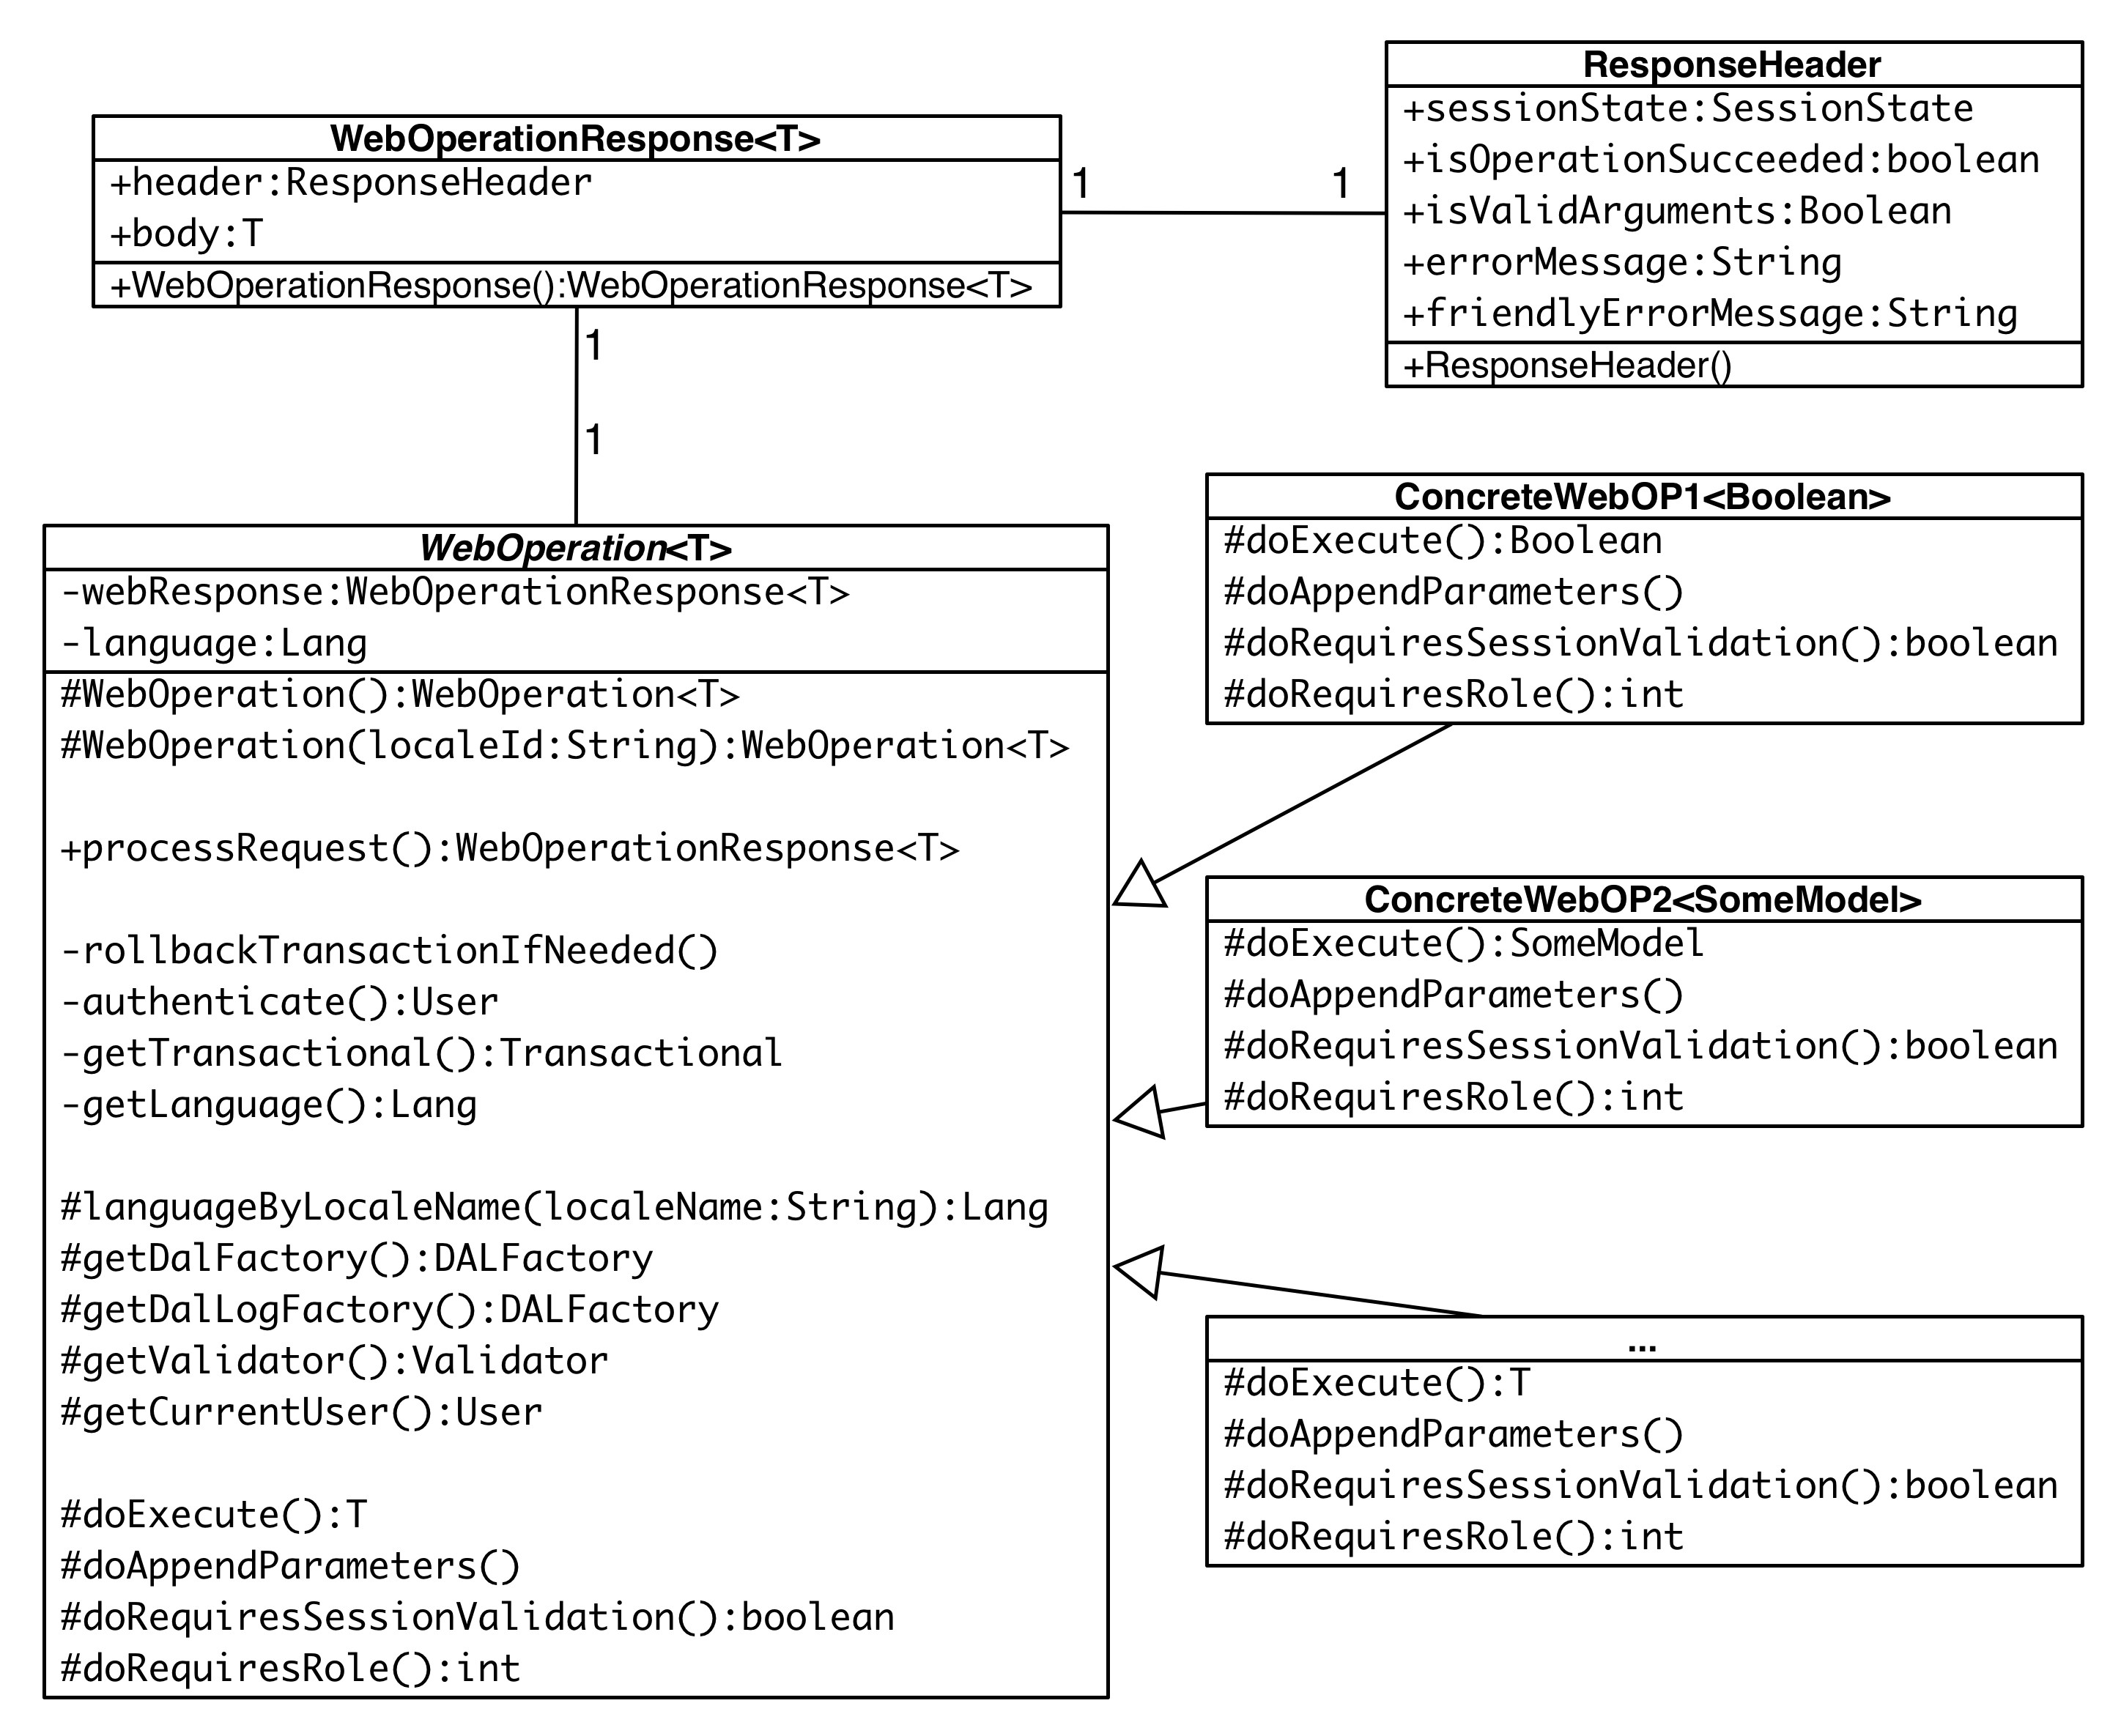
\includegraphics[width=13cm]{./images/umls/uml_diagram_api_core.jpg}
   \caption{UML diagram representing the core structure of the API.}
   \label{fig:umlAPICore}
\end{figure}
\\
The processing flow of the web operation is shown in Figure~\ref{fig:webOperationFlow}, which describes the actions taken by the  \verb"processRequest()" method:
\begin{figure}[h!]
 \centering
   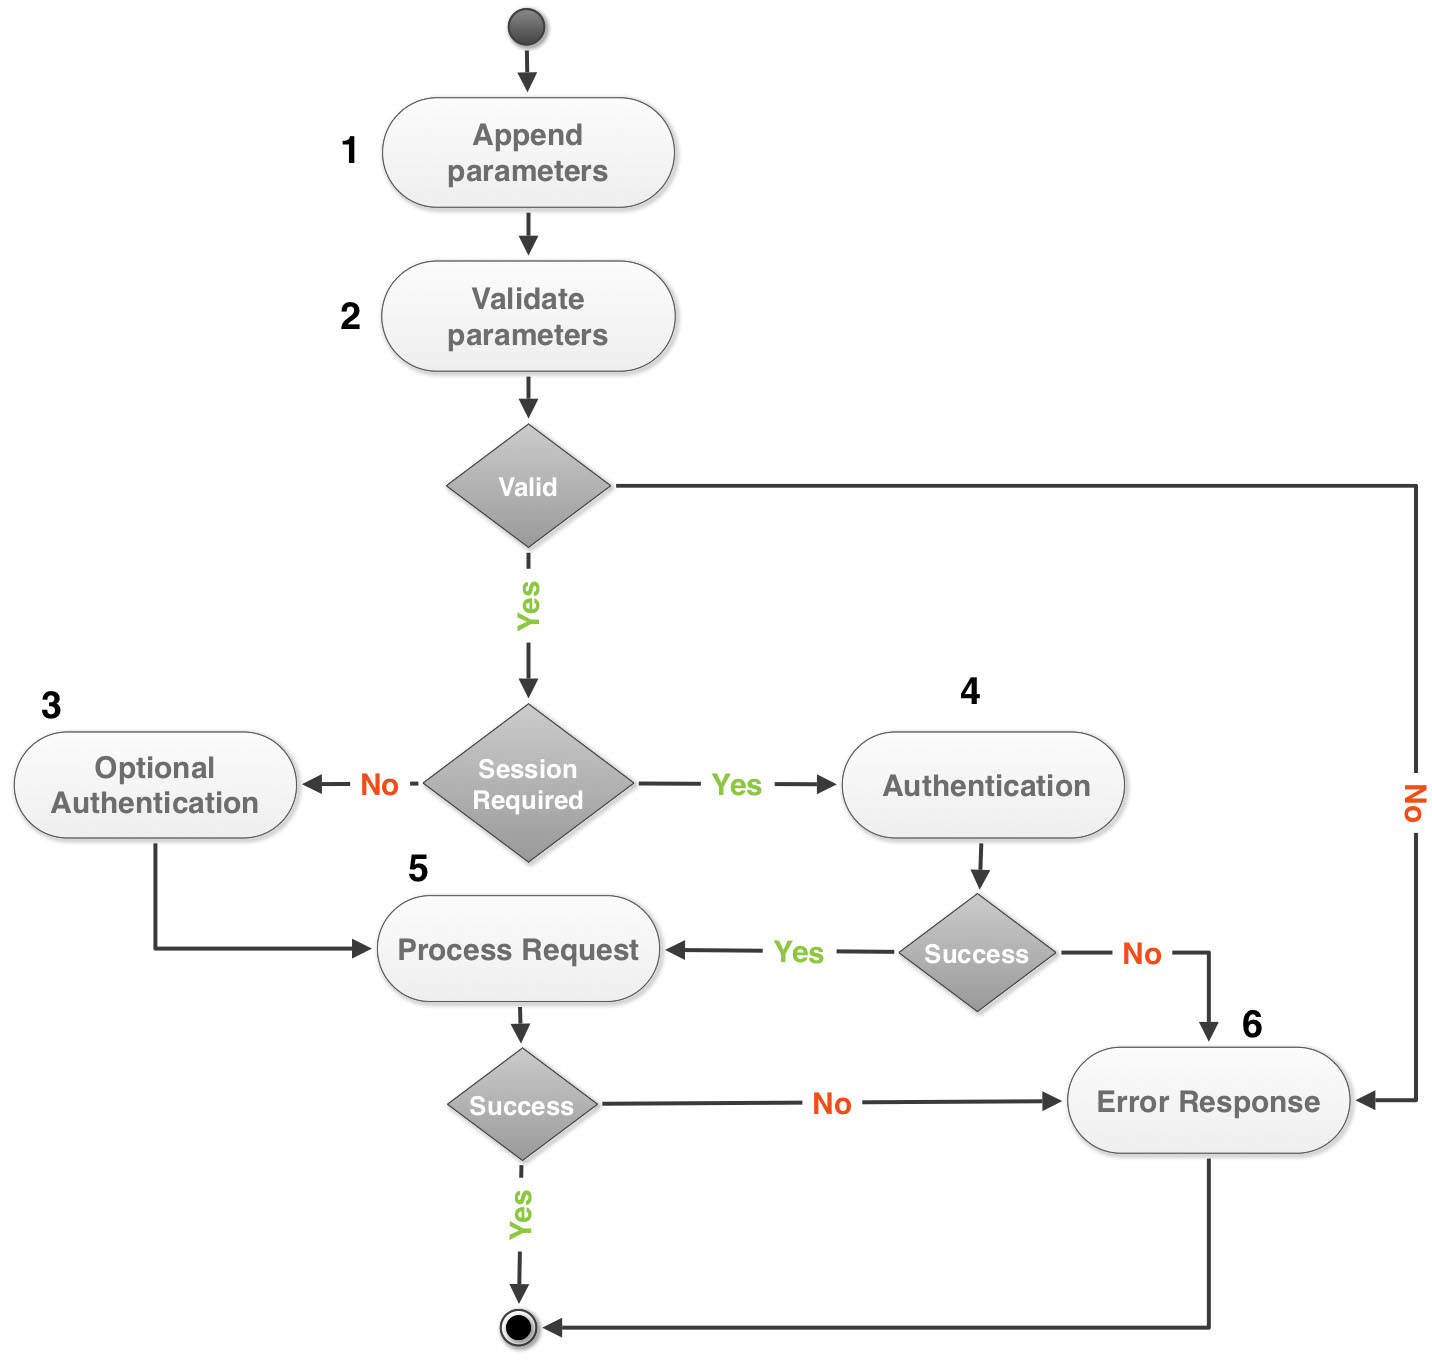
\includegraphics[width=9cm]{./images/flows/flow_web_operation_flow.jpg}
   \caption{Operation's validation and processing.}
   \label{fig:webOperationFlow}
\end{figure}
\begin{enumerate}
\item Concrete operation class adds the parameters to the validator.
\item Every parameter is validated to ensure that it is within the defined restrictions. If any of the parameters is invalid, the response header will contain the information explaining the error cause.
\item When the user authentication is optional, we verify if the sessionToken is passed, and if so, we fetch the user's information through the DAL. Any error that occurs during this phase is ignored. 
\item When user authentication is required, same actions are performed to retrieve the user information, but if any of these actions fails, the error response is generated.
\item The \verb"doExecute()" method from the child class is invoked, which is responsible for obtaining and processing the body of the response. If the operation succeeds, the response is populated with the result, otherwise it contains the information regarding the error content.
\end{enumerate}
If some unexpected error occurs during the \verb"processRequest()", through the DAL, its cause is registered to the log database for later analysis.\\
\\
Each web operation is implemented as a separate class which inherits the \verb"WebOperation<T>" where \verb"T" represents the type of the response upon the success. Every action delegates all the processing and validation to the respective instance of the \verb"WebOperation" and its endpoints path are in the \verb"conf/routes" configuration file. This file lists all the routes implemented by the API. Each route consists of an HTTP method and \gls{uri} pattern which are associated to an action method. The single route definition example is shown in Code Listing~\ref{cod:routeFile}.
\newpage
\begin{lstlisting}[language=java,caption={An example of the route file entry.},label={cod:routeFile}, frame=bt]
GET  /user/authenticate  controllers.User.authenticate(loc:String,tkn:String)
\end{lstlisting}
The responses of the web operation are serialised in \gls{json} format. When sent to user, the HTTP Header representing the \verb"content-type" is populated with \verb"application/json" value. The serialisation is achieved by using the  \gls{json} Jackson~\cite{jsonJackson} processor. During the development of the API we configured this framework to not serialize the attributes of the response when those are populated with \verb"null". The most direct example is the \verb"ResponseHeader", which excludes attributes presented in Code Listing~\ref{cod:optionalyProperties} when the response is successfully executed. Entities that represent information regarding the \verb"Location" and \verb"User" were also configured in the same manner.
\begin{lstlisting}[language=java,caption={Optional properties of the ResponseHeader.},label={cod:optionalyProperties}, frame=bt]
"errorMessage": null,
"validArguments": null,
"friendlyErrorMessage": null
\end{lstlisting}
This configuration allows to minimise the bandwidth occupied during the transmission of the response. With the illustrated example, we have spared 73 bytes, because that information would not be sent as part of the response, which equals to 1Mb for approximately each 15000 requests. For a large API usage, it will significantly minimise the amount of information to be sent from the server where the API is hosted and may increase the response time.
%%%%%%%
%%%%%%%
\subsection{Authentication}
\label{subsec:authentication}
Most of the implemented web operations retrieve data from the database through the DAL. But, the operations related to the authentication are different, since users can authenticate themselves on the service by using their Facebook~\cite{facebook} or Twitter~\cite{twitter} accounts. If the user exists, a session token is generated, allowing to execute API operations that require authentication. When the user authenticates himself by the first time, the service automatically creates a new account for that user. For the Facebook authentication, we use RestFB~\cite{restfb} framework that allows to obtain information regarding the users such as, name, email, among others fields. Then, the information is mapped directly to the Java classes. The framework provides an easy way to navigate through the Facebook Graph API~\cite{facebookGraphAPI}.\\
\\
Twitter's authentication service is managed in a similar way. To interact with the Twitter REST API v1.1~\cite{twitterRestAPI} we have used Twitter4j~\cite{twitter4j} library which already handles the authentication and provides wrappers to access user's information.\\
\\
Both services implement the authentication using the OAuth 2.0~\cite{oauth2} protocol. From the application side, the user should perform authorization using the preferred service. Then, the authorization data (token, token secret, and expiry date) is sent to our authorization endpoint and used to obtain information regarding the user in question. Finally, this information is used to populate the database with user's information and consequently perform the authentication.
%%%%%%%
%%%%%%%
\subsection{Location Creation}
\label{subsec:locationCreation}
During the location creation, users have to pick the location positioning coordinates from the map. When those are submitted to the service, the information regarding the location such as city, country, and address, are obtained automatically through the Reverse Geocoding~\cite{googleGeocodingAPI} process. The~\gls{gg}~\gls{api} is used for this purpose by allowing to extract human-readable address from a map location.\\
\\
The descriptive information regarding the address can be obtained in different languages. As of the time of this writing, the latest API version (v3) supports 55 different languages and dialects~\cite{googleGeocodingLanguages}. An example of a GG request (asking information about localization with latitude=38.76347 and longitude=-9.093783) is presented below:\\
\\
\verb"http://maps.googleapis.com/maps/api/geocode/json?latlng=38.763470,-9.093783&"\\
\verb"sensor=false&language=pt"\\
\\
Code Listing~\ref{cod:GoogleReverseGeocoddingJSON} shows an example of the~\gls{gg} response for the request presented above.
\begin{lstlisting}[language=json,firstnumber=1,caption={Google Geocoding JSON response example.},label={cod:GoogleReverseGeocoddingJSON}]
{
 "results" : [ {
     "address_components" : [
       {
         "long_name" : "Lisboa",
         "short_name" : "Lisboa",
         "types" : [ "locality", "political" ]
       },
       {
         "long_name" : "Portugal",
         "short_name" : "PT",
         "types" : [ "country", "political" ]
       },
       {...}
     ],
     "formatted_address" : "Passeio Ulisses 9, 2715-311 Lisboa, Portugal",
   },
   ...],
 "status" : "OK"
}
\end{lstlisting}
The \verb"language" attribute is the union of the ISO 639-1 and RFC 3066~\cite{rfc3066} standards, so its value is adapted according to the system language, which follows the ISO 639-1 format.
%%%%%%
%%%%%%
\subsection{Location Filtering}
\label{subsec:locationFiltering}
The REST API provides a set of methods that allow to perform different operations, such as authentication, lookup for points of interest, among others. There is a specific set of endpoints to perform the filtering of the touristic locations. Operations that obtain visited, recommended, and wanted locations are not subject to filtering criteria.\\
\\
Touristic location filtering can be achieved with \verb"/location/filter" endpoint where most of the arguments are optional. It allows to specify any combination of the arguments, easily adapting to user needs. It is possible to have any permutation of the filtering criteria such as city name, attraction, weather conditions, distance, among others.\\
\\
When the geographic coordinates pointing to user's current location are retrieved from the device, the latitude and longitude are passed to the service during the queries related to location filtering. We use this information to compute the distance between the user and location, presenting the results sorted increasingly by distance. For this purpose, we have used the Spherical Law of Cosines~\cite{sphericalCosine}, with the following set of equations:\\
\begin{equation}
  \begin{aligned}
    &\phi_{1} = userLat \times \frac{\pi}{180} \\
	&\phi_{2} = locationLat \times \frac{\pi}{180} \\
	&\Delta_\lambda = (userLon - locationLon) \times \frac{\pi}{180} \\
	&R\bigotimes = 6371\\
	\\
	&d = acos( sin(\phi_{1}) \times sin(\phi_{2}) + cos(\phi_{1}) \times cos(\phi_{2}) \times cos(\Delta_\lambda) ) \times R\bigotimes
  \end{aligned}
\end{equation}
where the $\phi_{1}$ represents user's latitude, $\phi_{2}$ refers to the location's latitude, and the $\Delta_\lambda$ is the difference between the user's and location's longitude coordinate. These values are converted to radians. The $R\bigotimes$ is a constant representing the distance in kilometres from Earth's center to its surface. The result $d$ represents the distance in kilometres between the user's specified coordinates and the touristic location at hand.

%%%%%%
%%%%%%
\subsection{Integration with World Weather Online}
\label{subsec:integrationWWO}
Users can preview the temperature when they are consulting the details of the chosen touristic location. For this purpose, we have made integration with the World Weather Online (WWO)~\cite{wwo} public API which allows to access current weather conditions. Their API allows to consult detailed information regarding the weather and supports different response formats, namely the~\gls{xml}, \gls{csv}, and JSON. We are only consulting the information regarding the weather condition and temperature, with the response being serialized into JSON format.\\
\\
The main reasons for choosing this service is that it doesn't require any commercial license, it can be used for personal and commercial purposes, and provides reliable information regarding current weather. The free version of this API is limited to 500 requests per hour.\\
\\
The weather conditions and the temperature are obtained using the geographic coordinates of the location in cause. When the information is successfully obtained, it is stored into the database and considered valid for the next 3 hours. This implies that subsequent requests for the location details will not trigger any call to the \gls{wwo} API, improving significantly the response time of our service and still provide the user with the updated and accurate weather information.\\
\\
Currently, the \gls{wwo} API supports around 48 different statuses for classifying the weather conditions~\cite{wwoCodes}. For this project, many of these statuses are not relevant, so we have shortened this set into 6 in order to represent the most common weather conditions. After querying the \gls{wwo} service, the weather condition value is converted into our domain specified value and our users are provided with minimalistic information regarding this matter. As an example, the \gls{wwo} API provides more than 15 statuses for classifying the rainy weather condition, when this information is received, it's mapped as \emph{rainy}, thereby minimizing the amount of redundant information. 

%%%%%%%%%%%%%%%%%%%%%%%%%%%%%%%%%%%%%%%%%%%%%%%%%%%%%%%%%%%%
\section{Recommender system}
\label{sec:recommenderService}
The Recommender system is one of the key features of the GuideMe service. In order to provide quality recommendations for our users, we have used the Apache Mahout Recommendation Engine library~\cite{apacheMahout}. Mahout provides a varied set of the Collaborative Filtering algorithms, for user and item based recommendations. Nowadays, this library is widely used for the implementation of recommendation systems.\\
\\
As we have described in Chapter~\ref{theory}, due to recommendation quality and algorithm performance benefits we have chosen the Item-Based Collaborative Filtering approach as our candidate for the recommender system. The implemented recommender system is implemented with the Slope One algorithm and scheduled with the Cron job to run every day at 3:00 AM. The chosen algorithm has proven to be fast, but overall performance has it's drawbacks when the datasource uses information from the database. To improve the performance of the recommendation system, we have imposed some restrictions which consist in selecting the users that should receive new recommendations. Through DAL, the service obtains a list of users who are eligible\footnote{By eligible users, we consider users that have visited at least one location.} for recommendations, and then for each user we apply the following equation:\\
\begin{equation}
PVu = VSR/TV,
\end{equation}
where $PVu$ is the percentage of the visited locations since last recommendation, for specific user $u$. $TV$ represents the total number of visited locations and $VSR$ refers to the number of the visited sights since last recommendation. The new recommendations are only computed if the user had an increase of $5\%$ of the visited locations. This selection allows to improve algorithm performance by excluding users that don't have new visited locations. We consider that the change on the number of visits below $5\%$ is meaningless regarding the recommendation results. Finally, we remove all previous recommendations and populate the database with new results.\\
\\
To accelerate the recommendation process by taking the advantage of the processing power, users eligible for new recommendations are divided into equal sets. Each set is passed to a different thread where the recommendations are computed and stored to the database.

%%%%%%%%%%%%%%%%%%%%%%%%%%%%%%%%%%%%%%%%%%%%%%%%%%%%%%%%%%%%
\section{Mobile Application}
\label{sec:iosApplication}
In this Section we describe the implementation aspects of the iOS mobile application, what kind of operations and features it offers and how those features were implemented. We start by detailing the communication layer between our service and iOS application. Then, we present the application overview, followed by aspects regarding the internationalization.\\
\\
The iOS application is implemented following the concept of universal app. A universal app is a single application that is optimized for iPhone, iPod touch, and iPad devices. The final product is a representation of a single binary that adapts to the current device. When searched on the App Store~\cite{appleAppStore} the same binary is shown for the iPhone/iPod and iPad devices instead of having different binaries for each device.\\
\\
The development of the universal binary involved extra work. Because of the differences in device screen sizes, most of windows, views, and view controllers code for iPad is different from the code for iPhone and iPod touch. In addition, there are some differences between interface principles in iPhone and iPad platforms, which are described along in iOS Human Interface Guidelines~\cite{appleiOSGuideLines}.\\
\\
Users usually prefer an universal app instead of a device-specific. They need to download it only once, and if an app is correctly designed, every additional feature that they activate is automatically enabled across all devices using the iCloud~\cite{appleiCloud} service.
%%%%%%%
%%%%%%%
\subsection{Communication Layer}
\label{subsec:iosCommunicationLayer}
A flexible interface for the communication with the service was designed to facilitate the developments of the iOS applications. Figure~\ref{fig:umliOSServiceLayer} shows the~\gls{uml} diagram describing the main classes responsible for the communication with the service infrastructure. Every concrete implementation of the model inherits the \verb"BaseModel" and implements the \verb"parserWithJson" method from the \verb"ParserProtocol". This method ensures that the model knows how to parse properties from the response serialized in \gls{json} format.
\begin{figure}[h!]
 \centering
   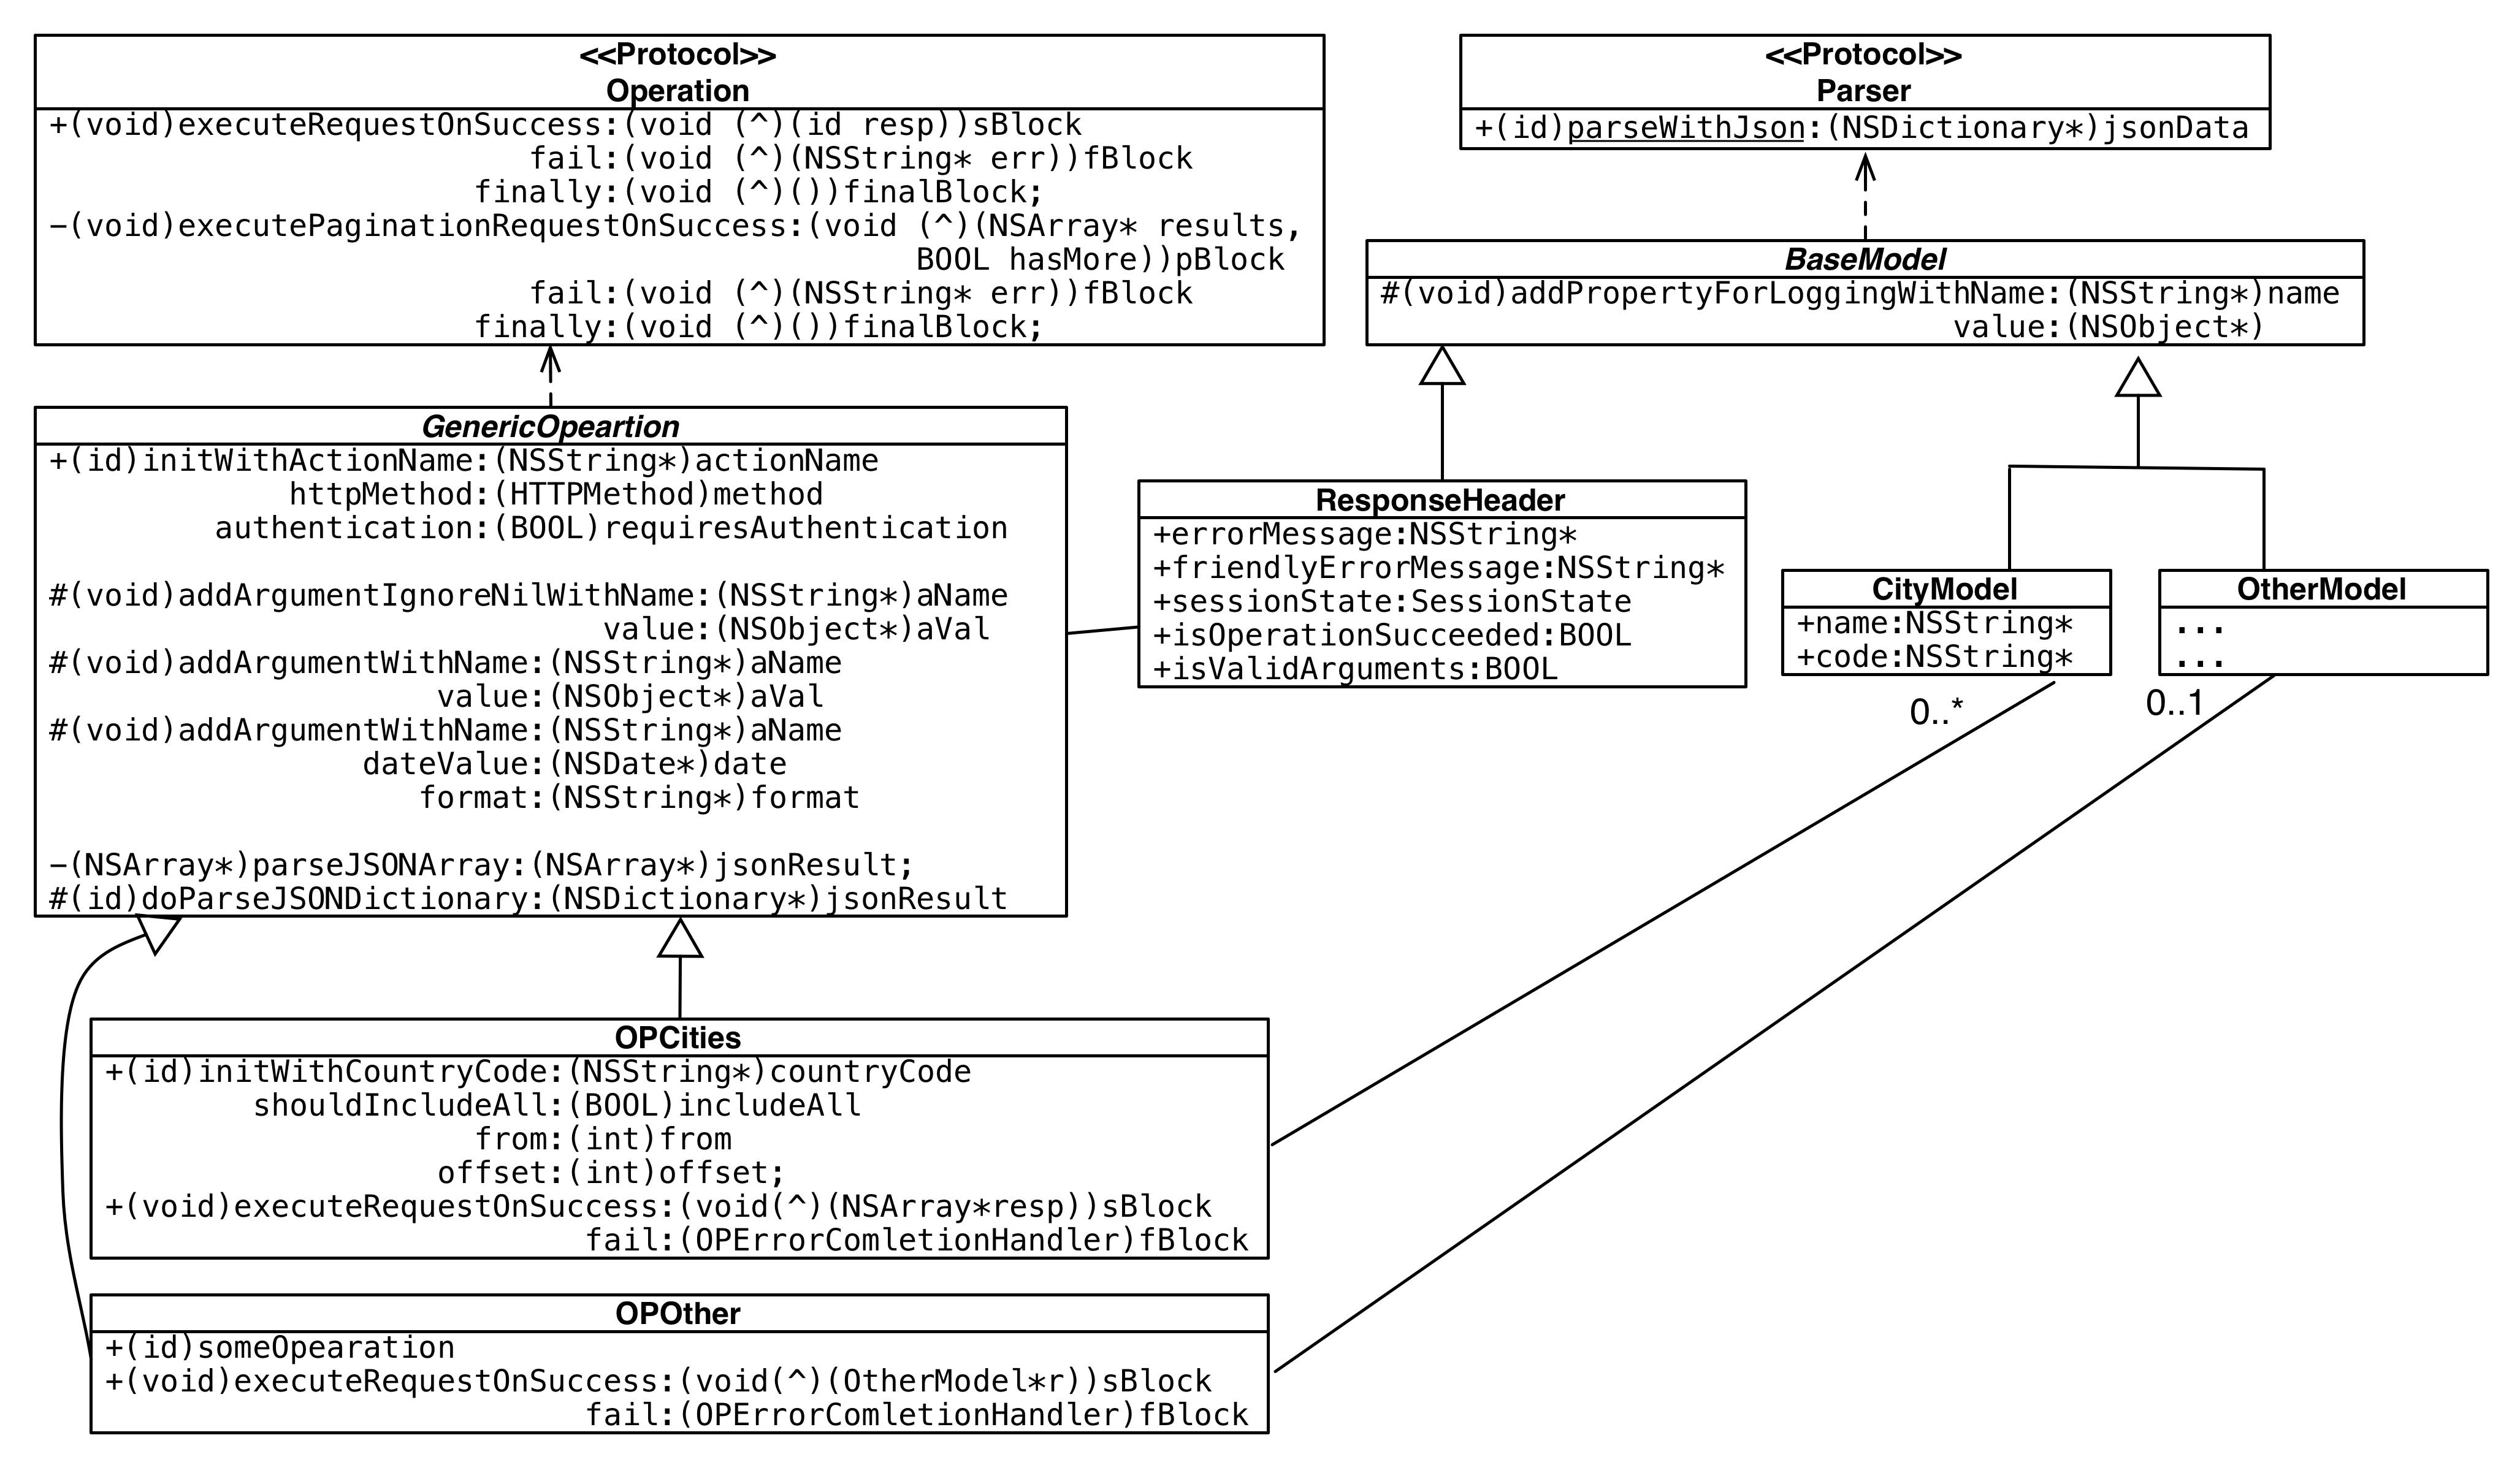
\includegraphics[width=11.8cm]{./images/umls/uml_diagram_ios.jpg}
   \caption{UML diagram representing the communication layer of the iOS application.}
   \label{fig:umliOSServiceLayer}
\end{figure}
\\
The \verb"GenericOperation" class is responsible for making the request to the endpoint defined by the child class. The request is executed as a background task using the~\gls{gcd}\footnote{\gls{gcd} comprises language features, runtime libraries, and system enhancements that provide systemic, comprehensive improvements to the support for concurrent code execution on multicore hardware in iOS and OS X~\cite{gcd}.}, which allows to execute the request asynchronously in a background thread. Figure~\ref{fig:iosExecutionFlow} illustrates the most important steps required to perform the remote request, which are detailed as follows:\\
\begin{enumerate}
\item The class that inherits the \verb"GenericOperation" specifies the endpoint and the HTTP method required to perform the operation.
\item The parameters are appended to the request.
\item The remote request is performed on a background thread.
\item When the response arrives, it is validated and parsed.
\item The failure block is invoked on the main thread when the response is invalid or the header is populated with information regarding an error.
\item The success block is called on the main thread if everything goes as expected.
\item If the user has specified the finally block, it will be executed on the main thread after the success or failure blocks.
\end{enumerate}
\begin{figure}[h!]
 \centering
   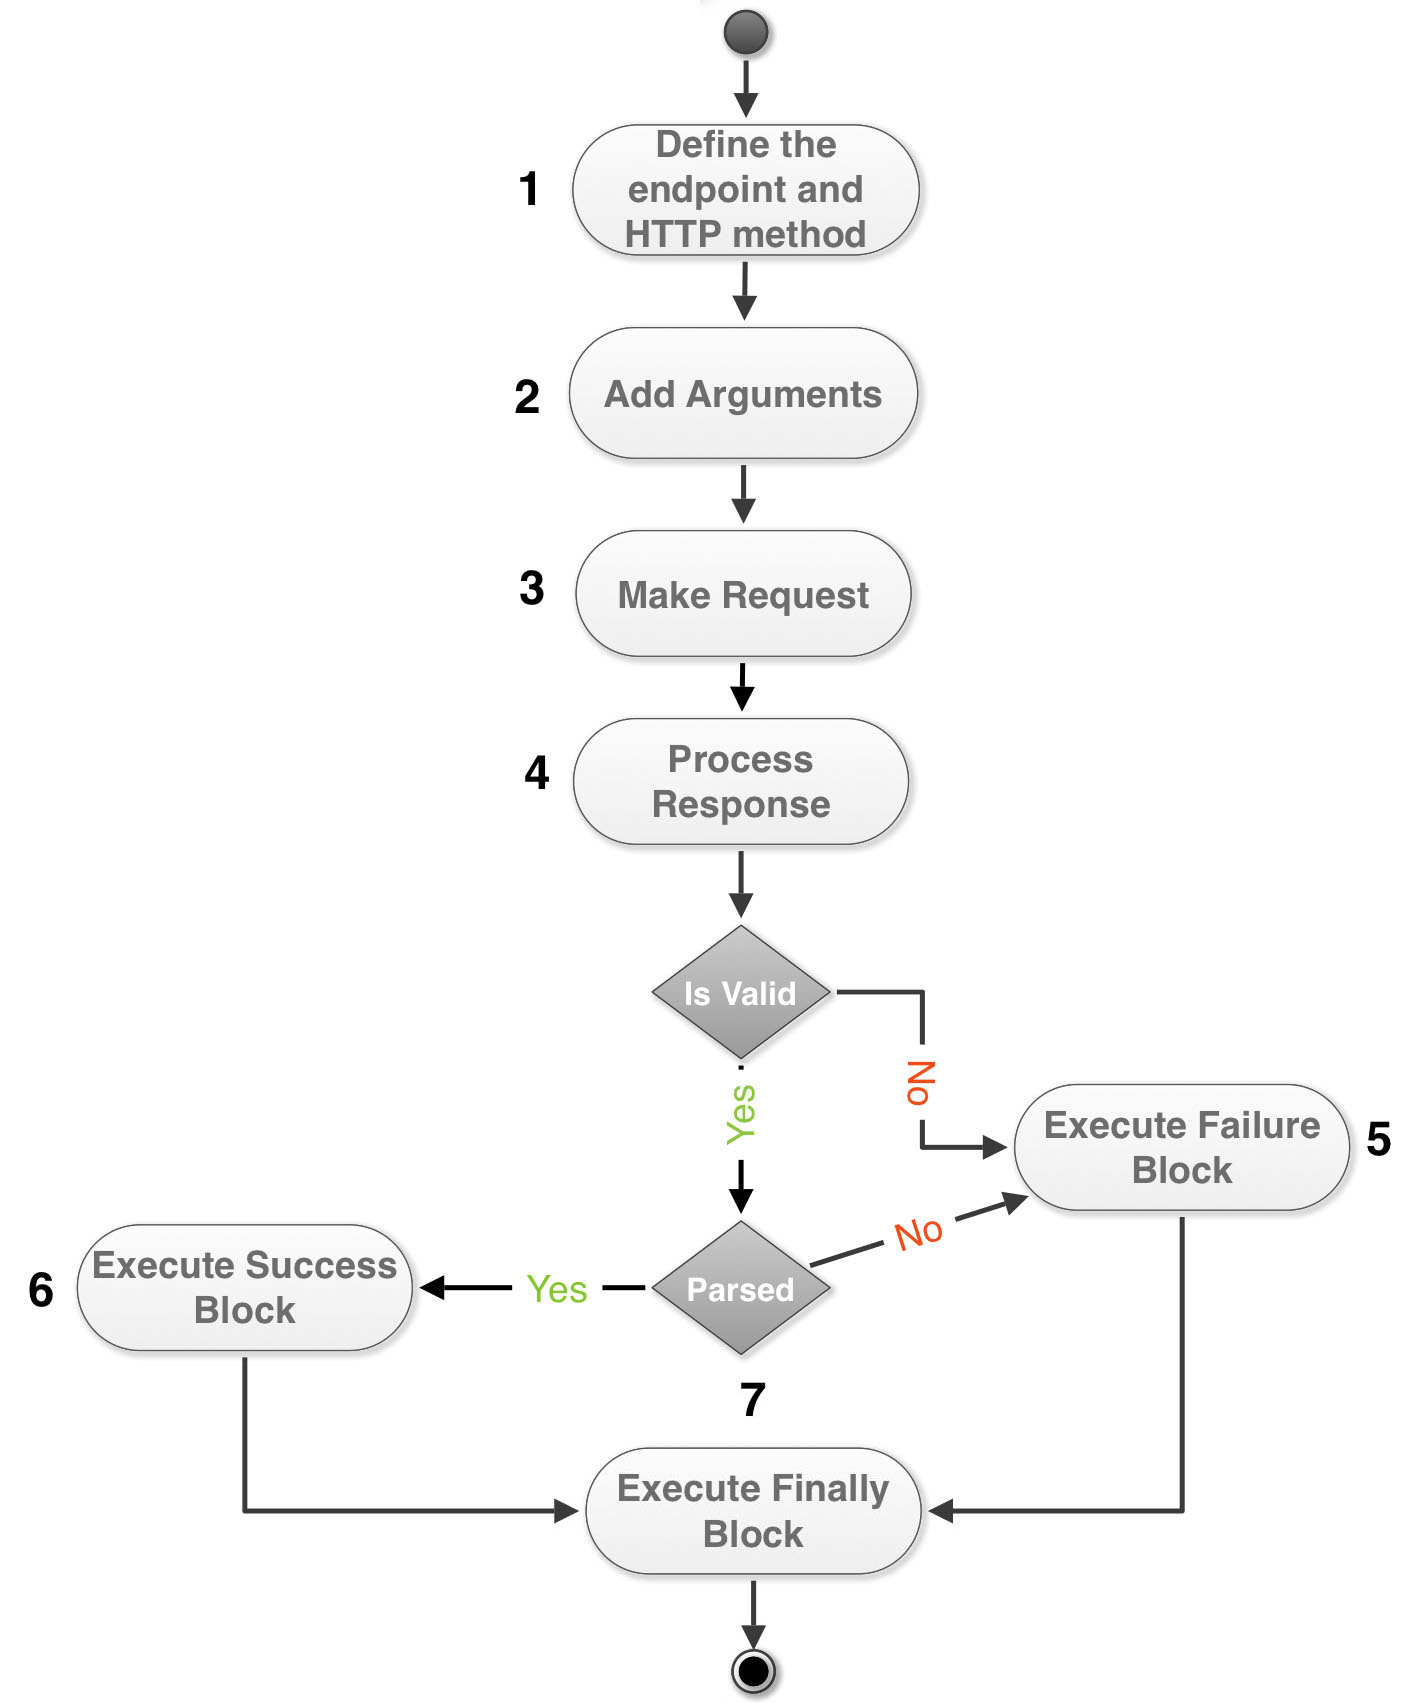
\includegraphics[width=9cm]{./images/flows/flow_ios_operation_flow.jpg}
   \caption{Processing of the remote request.}
   \label{fig:iosExecutionFlow}
\end{figure}
The implementation with blocks has simplified the usage of the classes that perform the remote requests. The current approach performs the background task to handle the request and invokes the described blocks on a main thread, allowing to implement the \gls{ui} operations directly inside the respective block. As a consequence, we minimise the amount of code to be written. Code Listing~\ref{cod:iosGCDCommonApproach} illustrates an example of the common implementation to perform such tasks in a background thread and then update the \gls{ui} on the main thread.\\
\begin{lstlisting}[language={[Objective]C},caption={An example of the remote request using common GCD approach.},label={cod:iosGCDCommonApproach}, belowskip=3em, frame=bt, ]
dispatch_queue_t getCitiesQueue = dispatch_queue_create("get cities", NULL);
   dispatch_async(getCitiesQueue, ^(){
      NSError ** error;
      NSArray * cities = [CitiesOP performOperationWithCountryCode:@"PT" 
                          shouldIncludeAll:NO from:0 count:10 error:&error];
      dispatch_async(dispatch_get_main_queue(), ^(){
         if(!cities){ /* Notify user about the error */ }
         else{        /* Handle the "cities" response here */ }
         // Perform some common operations
         });
});
\end{lstlisting}
The adopted solution, shown in Code Listing~\ref{cod:iosGCDImproovedApproach} simplifies the readability and amount of code to be written. The scheduling to the background thread and the main thread are made internally by the implemented infrastructure.\\
\begin{lstlisting}[language={[Objective]C},caption={An example of the remote request using the adopted solution.},label={cod:iosGCDImproovedApproach}, frame=bt]
OPCities *citiesOP = [[OPCities alloc] initWithCountryCode:@"PT" 
                                          shouldIncludeAll:NO 
                                                      from:0 
                                                     count:100];
[citiesOP executeRequestOnSuccess:^(NSArray *cities){
   // Handle the "cities" response here
 } fail:^(NSString *errorMessage){
   // Notify the user about the occurred error
 } finally:^(){
   // Implementation of some common actions
}];
\end{lstlisting} 
%%%%%%%
%%%%%%%
\subsection{iOS Application Overview}
\label{subsec:ioHighlightedFeatures}
The developed mobile application offers two interfaces. The common interface which can be accessed by any user and the interface for administration.
All users can consult points of interest near their current location, apply filtering criteria (e.g. filtering by country, city, category, weather conditions, among others) to shorten the amount of results. Users also have the possibility to consult recommended locations, mark locations as visited or wanted, follow and unfollow other users.\\
\\
Users with the administrative privileges have access to all of the described tasks. They can also insert new or update an existing touristic location, and consult information regarding the reported touristic locations. The main focus of the mobile applications is the users's current location, which is represented by the geographic coordinates obtained using the positioning service available on the user's device, such as~\gls{gps} or Wi-Fi. By knowing the users's current location, the service can compute the distance between the touristic location and the user's location, as discussed before (Subsection~\ref{subsec:locationFiltering}). When the location services are not available, the service continues to allow consulting of the points of interest but without the indication of the distance between the user and the touristic location at hand.\\
\\
Figure~\ref{fig:guideMeWebScreenshotsIOSFull} illustrates some of the implemented features of the application for iPhone.
\begin{figure}[h!]
\begin{center}
		\centering
        \begin{subfigure}[b]{0.30\textwidth}
	     		\centering
                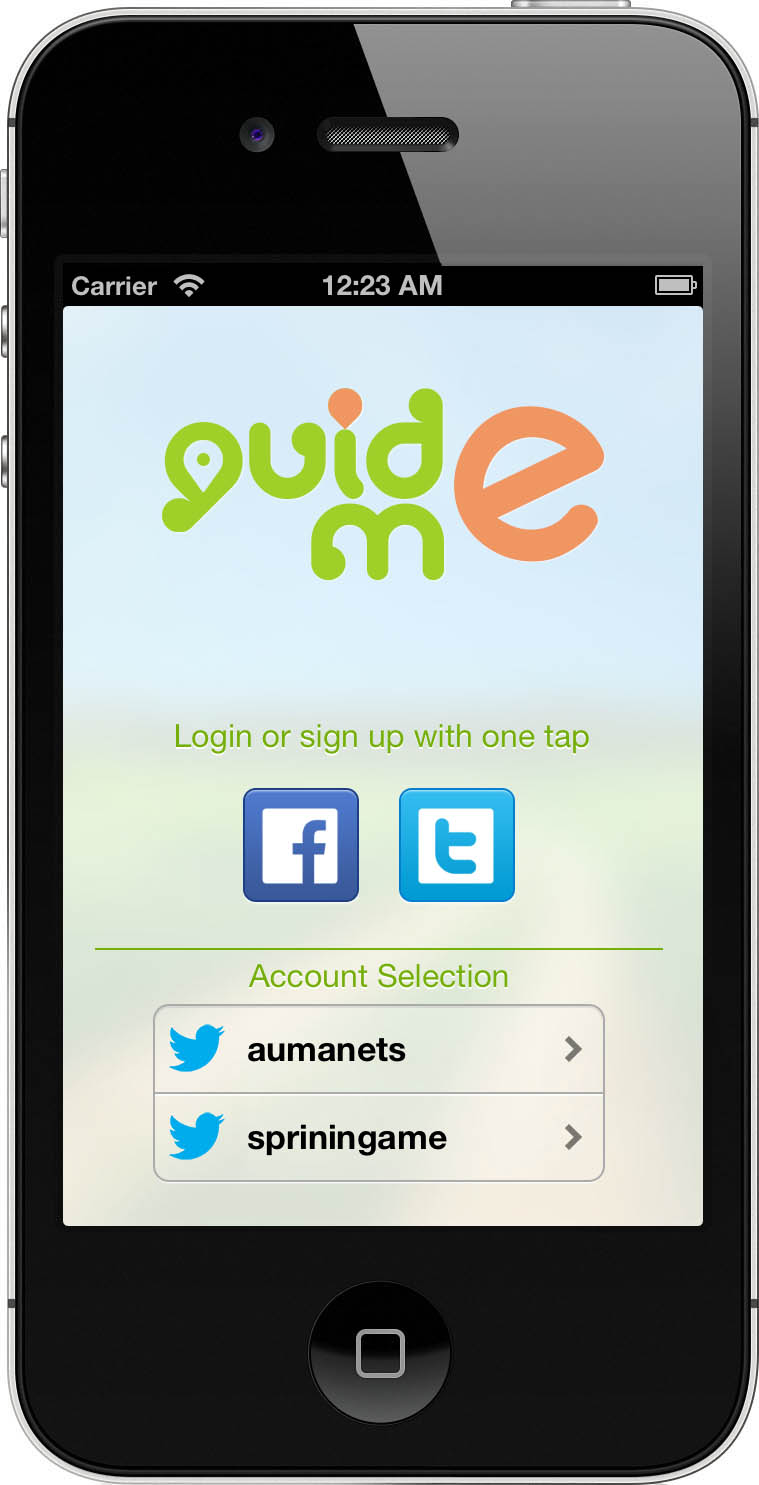
\includegraphics[height=8cm]{./images/screenshots/screenshot_iphone_app_1.jpg}
                \caption{Login screen.}
                \label{fig:guidemeWebScreenshotsIOSFina1}
        \end{subfigure}%
        \begin{subfigure}[b]{0.30\textwidth}
 				\centering
                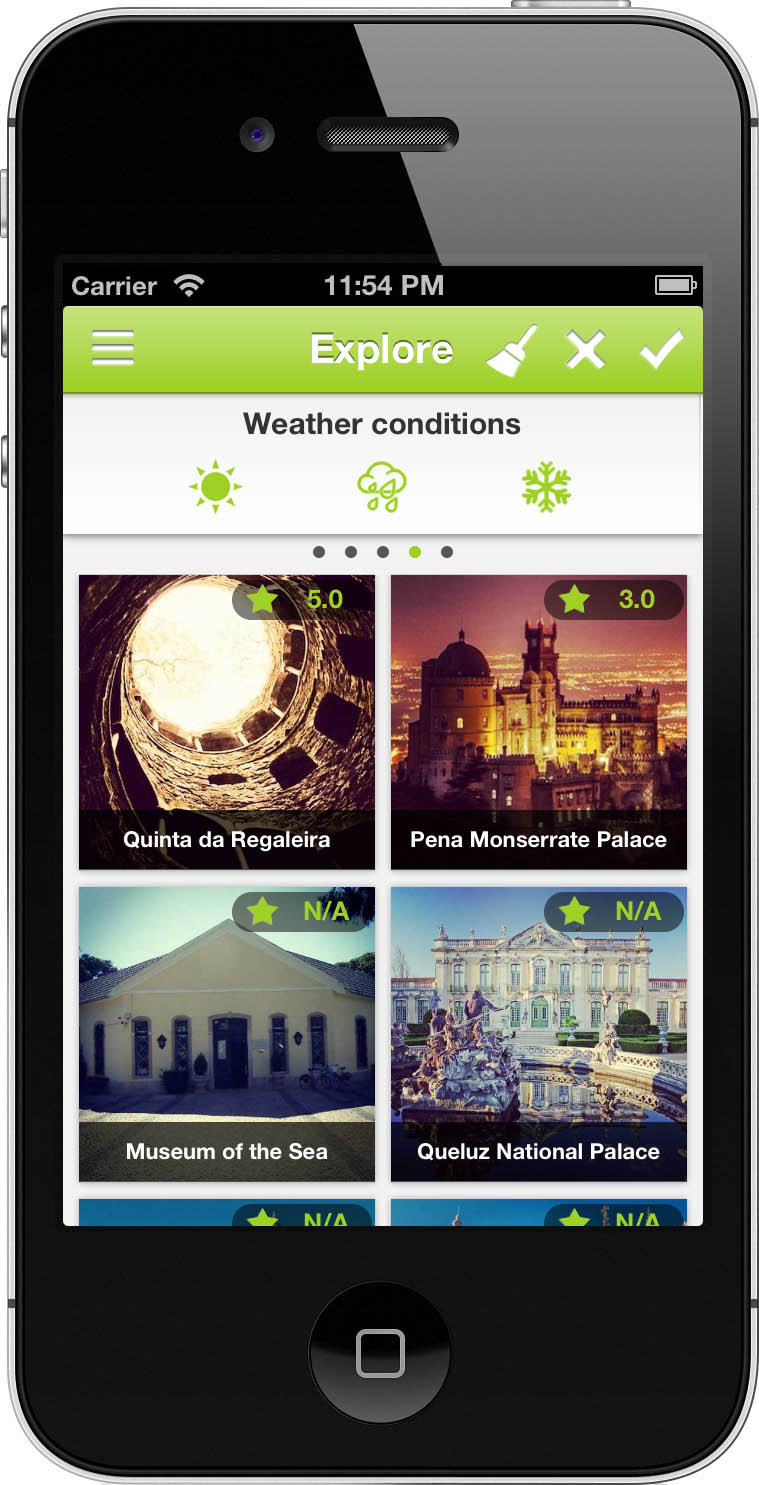
\includegraphics[height=8cm]{./images/screenshots/screenshot_iphone_app_2.jpg}
                \caption{Location search.}
                \label{fig:guidemeWebScreenshotsIOSFina2}
        \end{subfigure}
        \begin{subfigure}[b]{0.30\textwidth}
 				\centering
                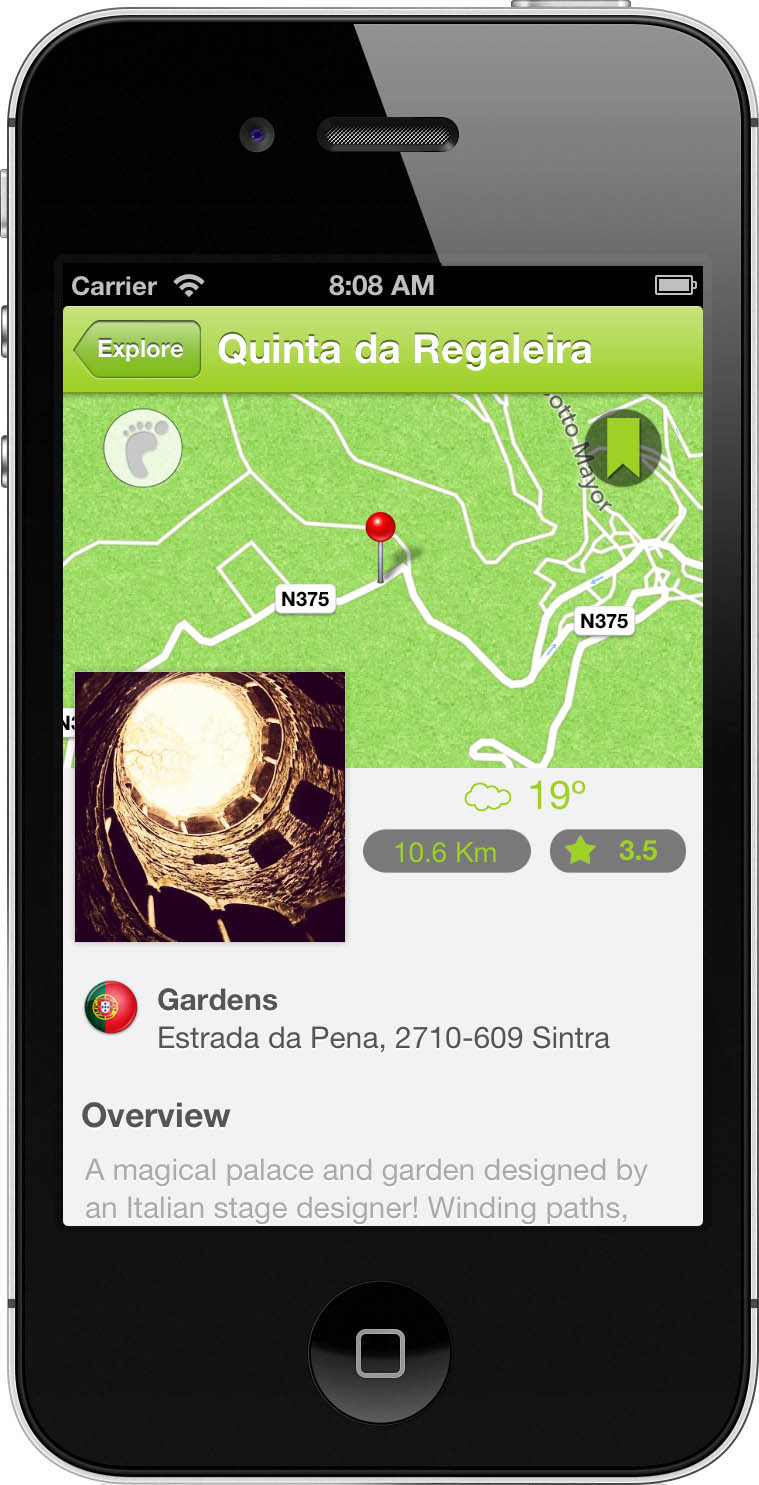
\includegraphics[height=8cm]{./images/screenshots/screenshot_iphone_app_3.jpg}
                \caption{Location details.}
                \label{fig:guidemeWebScreenshotsIOSFina3}
        \end{subfigure}
        \caption{Screenshots of the iPhone application}
        \label{fig:guideMeWebScreenshotsIOSFull}
        \end{center}
\end{figure}
In Figure~\ref{fig:guideMeWebScreenshotsIOSFull}~(\subref{fig:guidemeWebScreenshotsIOSFina1}) we have the login screen, where the user may choose the preferred social service in order to perform login or sign up. Figure~\ref{fig:guideMeWebScreenshotsIOSFull}~(\subref{fig:guidemeWebScreenshotsIOSFina2}) shows a list of the locations, which have resulted from the applied filtering criteria. The detailed information regarding the chosen location is presented in a similar way as illustrated in Figure~\ref{fig:guideMeWebScreenshotsIOSFull}~(\subref{fig:guidemeWebScreenshotsIOSFina3}).\\
\\
As it was previously stated, the iPad device is also supported by the application. In Figure~\ref{fig:guideMeWebScreenshotsiPadFull}~(\subref{fig:guidemeWebScreenshotsiPadFina1}) we have a screen with a list of the touristic locations and Figure~\ref{fig:guideMeWebScreenshotsiPadFull}~(\subref{fig:guidemeWebScreenshotsiPadFina2}) depicts the screen with detailed information of the selected location. It is clearly visible that the content of each screen is adapted to the device resolution and differs from the one presented in Figure~\ref{fig:guidemeWebScreenshotsIOSFina3}~(\subref{fig:guidemeWebScreenshotsIOSFina2}) and Figure~\ref{fig:guidemeWebScreenshotsIOSFina3}~(\subref{fig:guidemeWebScreenshotsIOSFina3}). Both implementations share the same code with a few adjustments that distinguish the iPhone version from the iPad (universal application).\\
\begin{figure}[h!]
\begin{center}
		\centering
        \begin{subfigure}[b]{0.45\textwidth}
 				\centering
                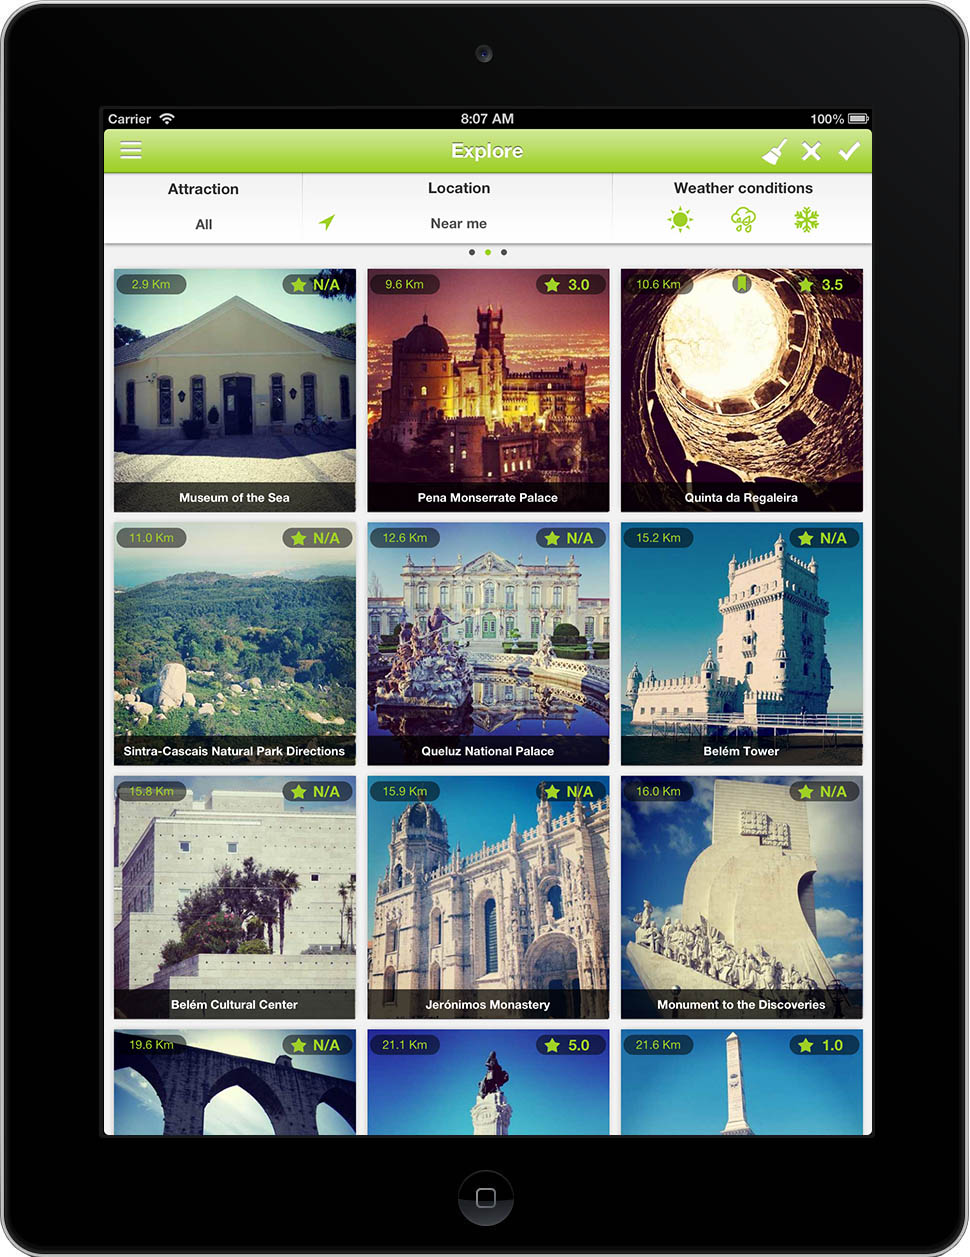
\includegraphics[height=8cm]{./images/screenshots/screenshot_ipad_app_1.jpg}
                \caption{Location search.}
                \label{fig:guidemeWebScreenshotsiPadFina1}
        \end{subfigure}
        \begin{subfigure}[b]{0.45\textwidth}
 				\centering
                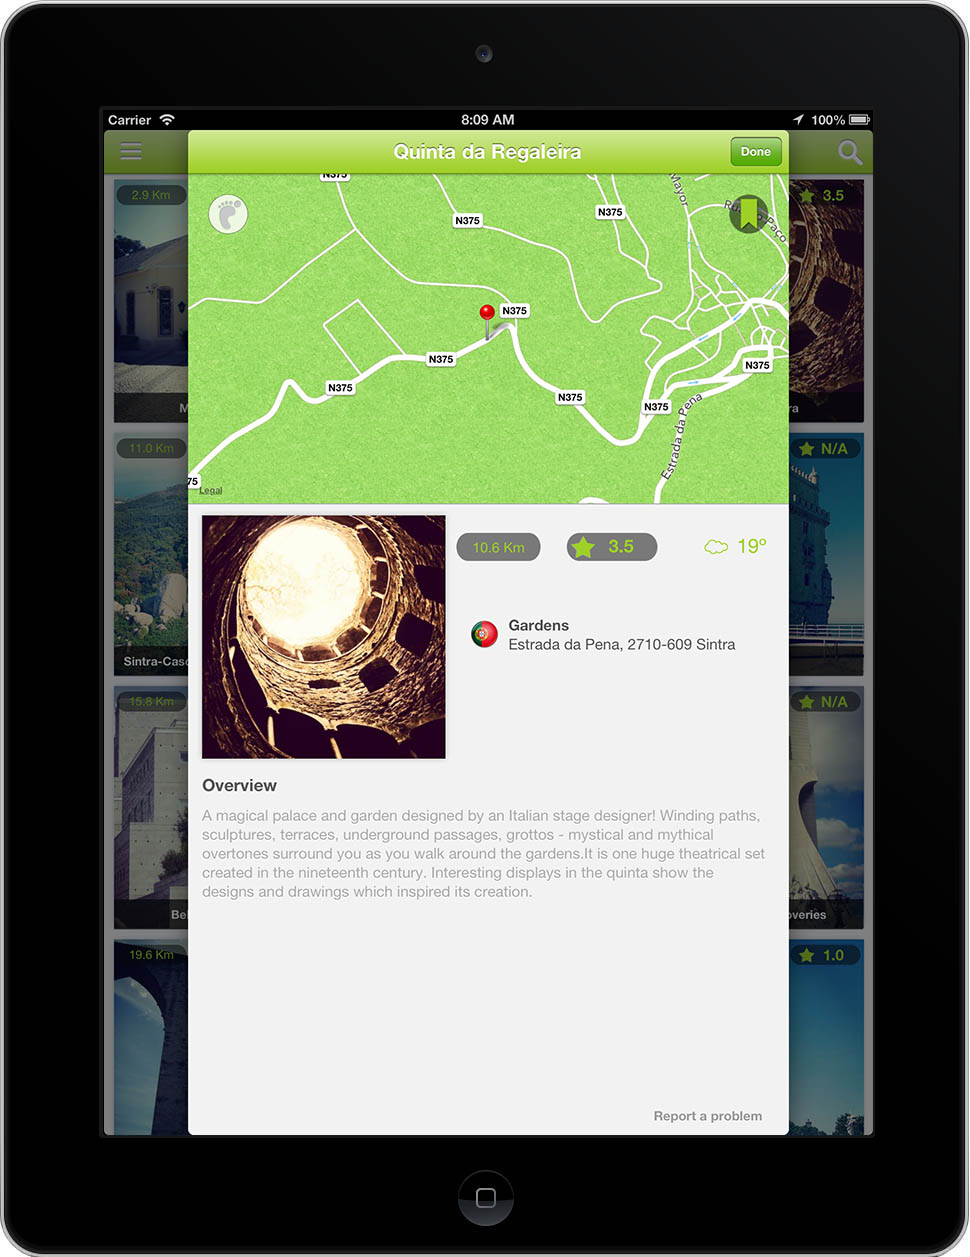
\includegraphics[height=8cm]{./images/screenshots/screenshot_ipad_app_2.jpg}
                \caption{Location details.}
                \label{fig:guidemeWebScreenshotsiPadFina2}
        \end{subfigure}
        \caption{Screenshots of the iPad application}
        \label{fig:guideMeWebScreenshotsiPadFull}
        \end{center}
\end{figure}\\
The full set of features for each version of the application is documented and located in the \emph{GuideMeMobileClient} repository.
%%%%%%%
%%%%%%%
\subsection{Internationalization}
\label{subsec:iosInternationalization}
The developed application provides translation strings for the English and Portuguese languages. If the user has configured any language other than English or Portuguese, the application assumes English by default. During the remote requests, the language identifier\footnote{The language identifier in the iOS application is defined in ISO 639-1 format. The same type of locale identifiers is supported by the REST API.} used for loading localized resources is passed to our REST API, ensuring that the information is retrieved using the same locale as the one configured by the device.

%%%%%%%
%%%%%%%
\section{Push Notifications}
\label{subsec:pushNotificationIntro}
We use the~\gls{apns} service to notify users about important events that occur regarding them. A use case of this concept, is when the user is followed by another, the push notification is sent detailing the occurred event as illustrated on Figure~\ref{fig:pushNotificationExamle}, otherwise this action could pass unnoticeable to the followed user.\\
\begin{figure}[h!]
 \centering
   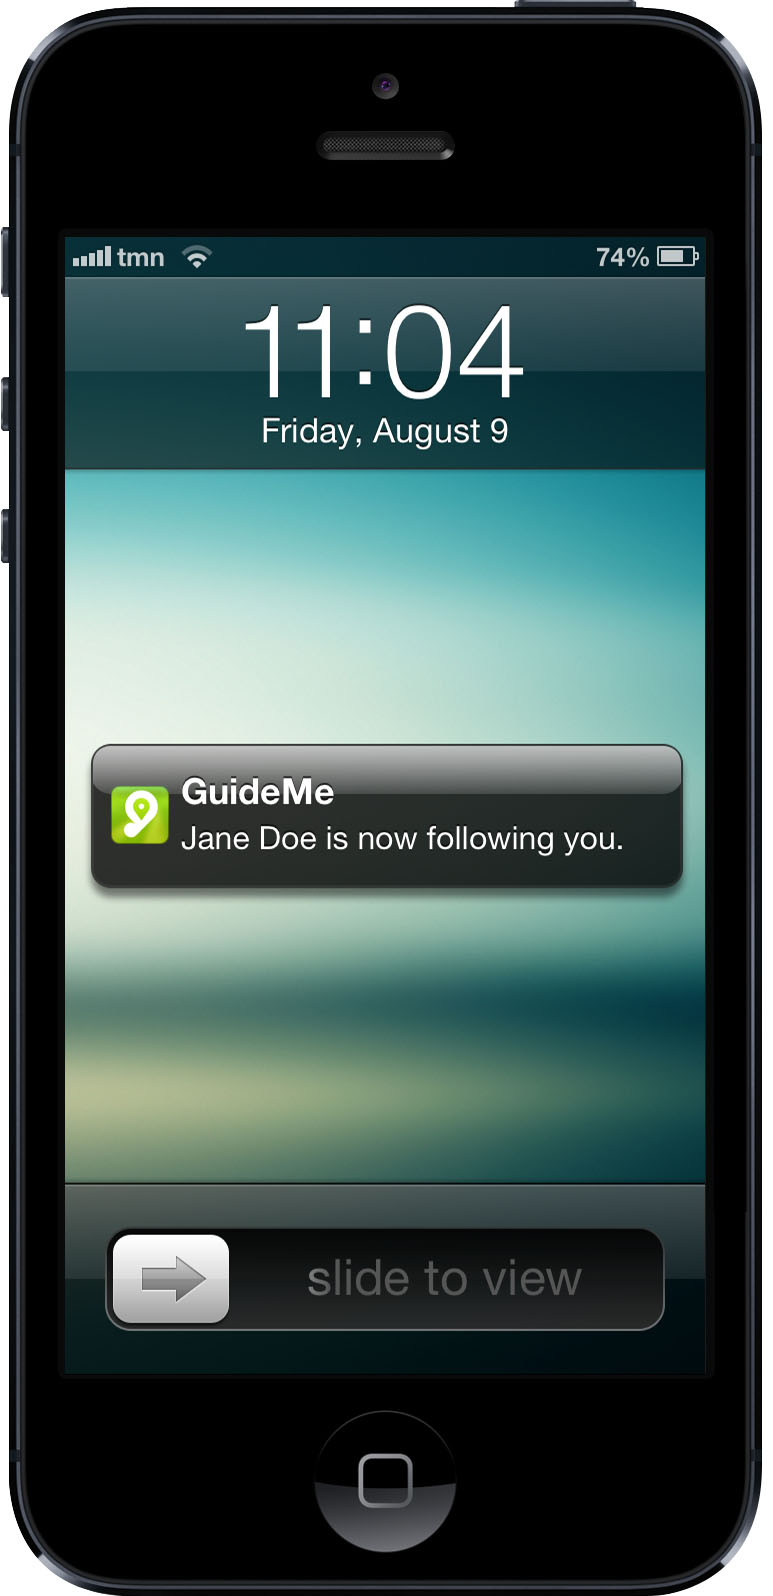
\includegraphics[height=6cm]{./images/screenshots/screenshot_push_notification_example.jpg}
   \caption{An example of the push notification sent by GuideMe service.}
   \label{fig:pushNotificationExamle}
\end{figure}\\
To implement this feature, we have used the Java-APNS~\cite{javaApns} implementation that already solves many of the difficulties, such as, communication with the APNS, establishing of a secure connection, among others. In order to make the provider communicate with the APNS and later the APNS with the device, it was required to correctly configure the certificate in Java-APNS framework and the Provisioning Profile~\cite{appleRemoteNotifProvisioning} during the deployment of the mobile applications\footnote{To develop and deploy the provider side of an application for push notifications, it is required  to obtain the SSL certificates from the appropriate Apple Developer Center~\cite{appleIosDeveCenter}.}. Each certificate is limited to a single application, identified by its bundle ID. It is also limited to one of two environments: development or production. These environments have their own assigned IP address and require their own certificates. It is also required to obtain provisioning profiles for each of these environments in order to receive the push notification when the application is deployed to the mobile device. The communication flow for sending the push notification, between the source and destination devices, is illustrated on Figure~\ref{fig:apnsUseCase}.\\
%%%%%%
\begin{figure}[h!]
 \centering
   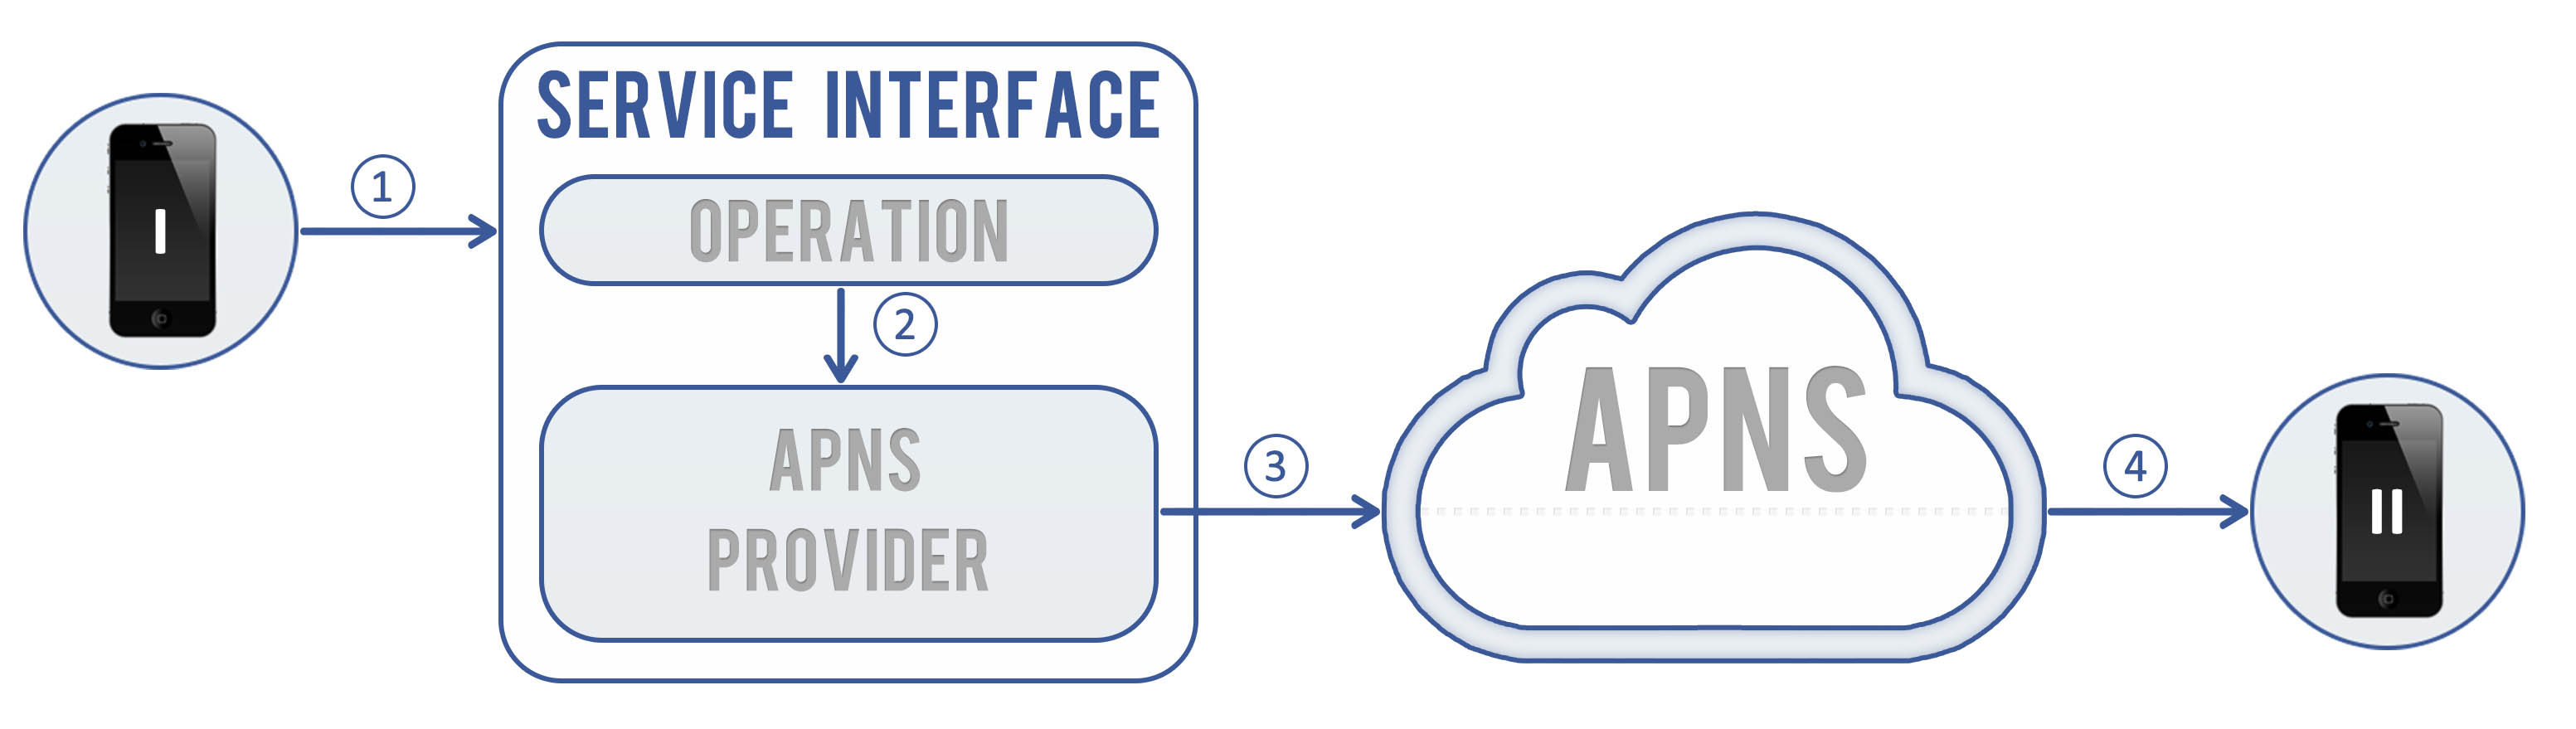
\includegraphics[height=2.8cm]{./images/diagrams/diagram_usecase_pushnotification.jpg}
   \caption{Delivery of the push notification to the destination device.}
   \label{fig:apnsUseCase}
\end{figure}\\
%%%%%%
The steps regarding the push notification delivery are as follows:
\begin{enumerate}
	\item The source device performs a remote request to execute an action (for example, follow some user).
	\item After a successfully performed operation, the routine from the APNS provider is invoked.
	\item A new notification is created and sent to the APNS server. 
	\item When possible, APNS delivers the notification to the destination device.
\end{enumerate}
%%%%%%
As it is stated by Apple, the provider is responsible for not propagating push notifications to devices that are not able to receive them. We have implemented a service, that is executed by Cron job every 10 minutes. This service connects to the APNS Feedback service and obtains the device tokens that have repeatedly reported failed-delivery attempts. Then, we update the database by deactivating the reported device tokens. This periodic service was implemented using the Java-APNS framework and uses the data access layers to update the status of the device token or report errors to the log database when it is necessary.
        
\section{Web Application}
\label{sec:mobileApp}
In this Section, we describe the development aspects of the Web application. We detail the features and functionalities offered by this application.
%%%%%%%%%%
\subsection{Implementation Details}
\label{subsec:webAppImplementation}
The Web application was developed using the same framework as the REST API. Play Framework offers powerful Scala\footnote{Scala is an object-functional programming and scripting language for general software applications, statically typed, designed to concisely express solutions in an elegant, type-safe and lightweight manner.} template engine which was inspired by ASP.NET Razor~\cite{aspNetRazor}. The template system was designed in a manner that facilitates the development of the web applications, where the \verb"'@'" character indicates the Scala statement and it does not require to explicitly close the code-block. An example of the template engine is shown in Code Listing~\ref{cod:playWebExample}.\\
\begin{lstlisting}[language=HTML,caption={An example of the Scala template.},label={cod:playWebExample}, frame=bt, belowskip=3em]
@(location: LocationModel)
@if(location == null){
   <h1>Location is invalid</h1>
}else{
   <h2>location.getTitle()</h2>
   <ul>
      @for(user <- location.visitedBy()) { <li>@user.name</li> }
   </ul>
}
\end{lstlisting} 
%%%%%%%
The Play application follows the~\gls{mvc} architectural pattern applied to the Web architecture. This pattern splits the application into separate layers: the Presentation layer and the Model layer. The Presentation layer is further split into a View and a Controller layer. The Model holds the domain-specific representation of the information on which the operation executes. The View renders the model into a form suitable for interaction, while the Controller responds to the~\gls{http} Requests and applies changes to the underlying model. The Views are designed using the Bootstrap~\cite{twitterBootstrap} which is designed for faster and easier Web development. It defines a set of generic components and layouts which are used across the application and removes the compatibility barrier between different browsers.
%%%%%%%%%%
%%%%%%%%%%
\subsection{Web Application Overview}
\label{subsec:webAppOveriew}
The Web application implements a subset of functionalities of the mobile application. It allows to users authenticate using their Facebook account, consult visited, wanted and recommended locations, and the detailed information of each location. They can visualize their profile page with the information regarding the current account. On the details page of the touristic point, users can consult the exact location through the Google Maps service.\\
\\
The Figure~\ref{fig:guideMeWebScreenshotsFull}~(\subref{fig:guidemeWebScreenshotsFina1}) illustrates the page with a set of visited locations. By selecting any of the listed locations, its details are shown in a similar way as one from Figure~\ref{fig:guideMeWebScreenshotsFull}~(\subref{fig:guidemeWebScreenshotsFina2}).
\begin{figure}
        \begin{subfigure}[b]{0.5\textwidth}
                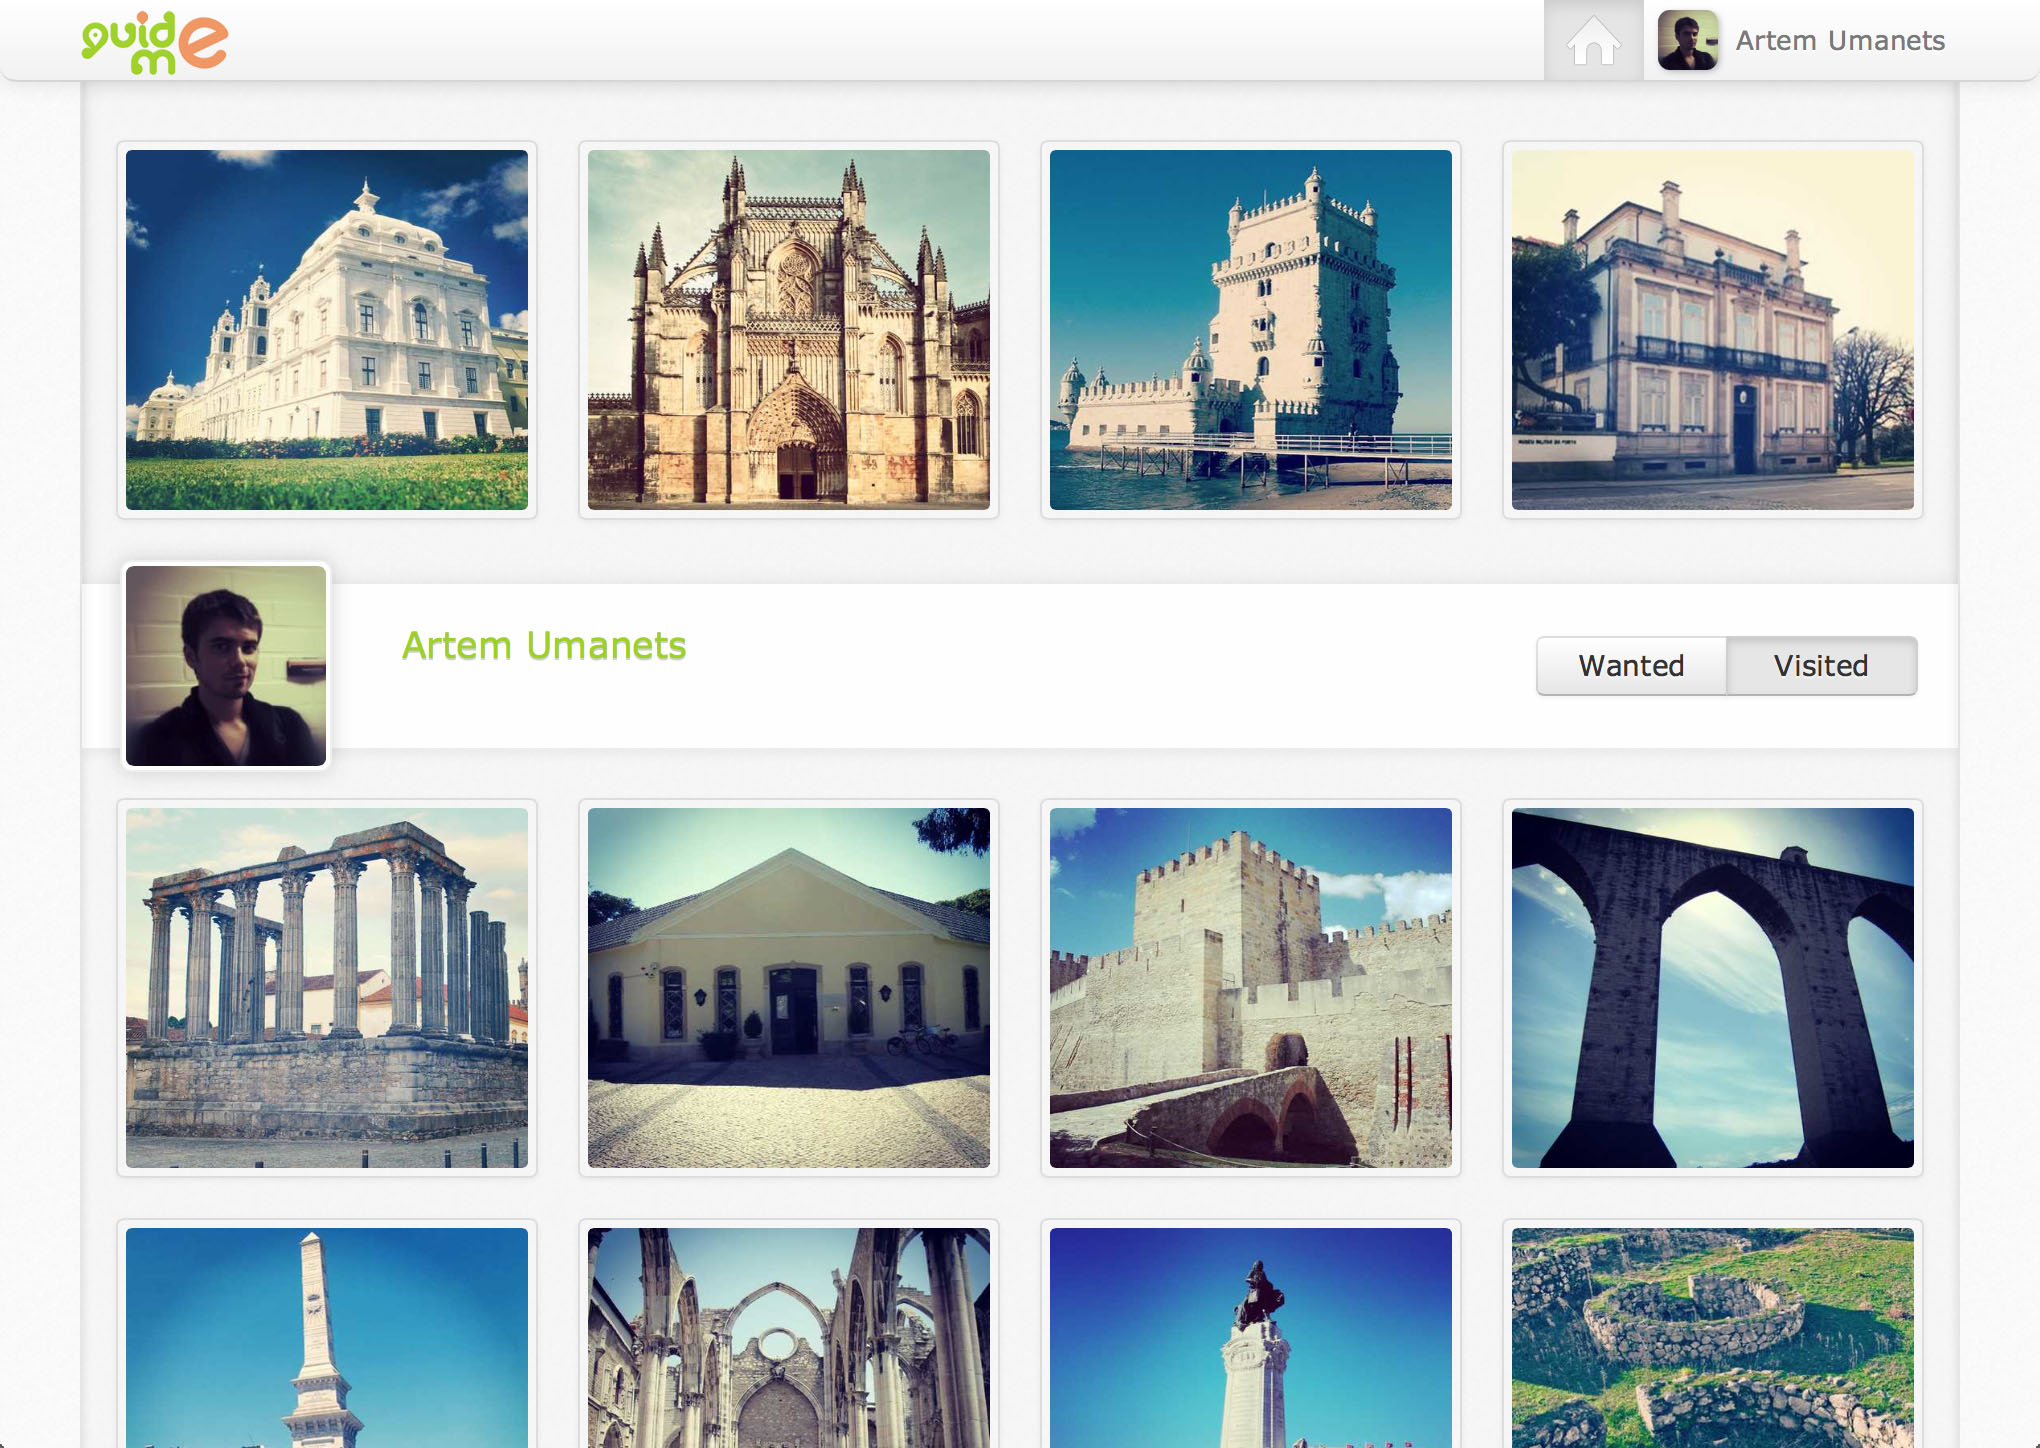
\includegraphics[height=5.2cm]{./images/screenshots/screenshot_web_app_1.jpg}
                \caption{Visited locations.}
                \label{fig:guidemeWebScreenshotsFina1}
        \end{subfigure}%
        \begin{subfigure}[b]{0.5\textwidth}
                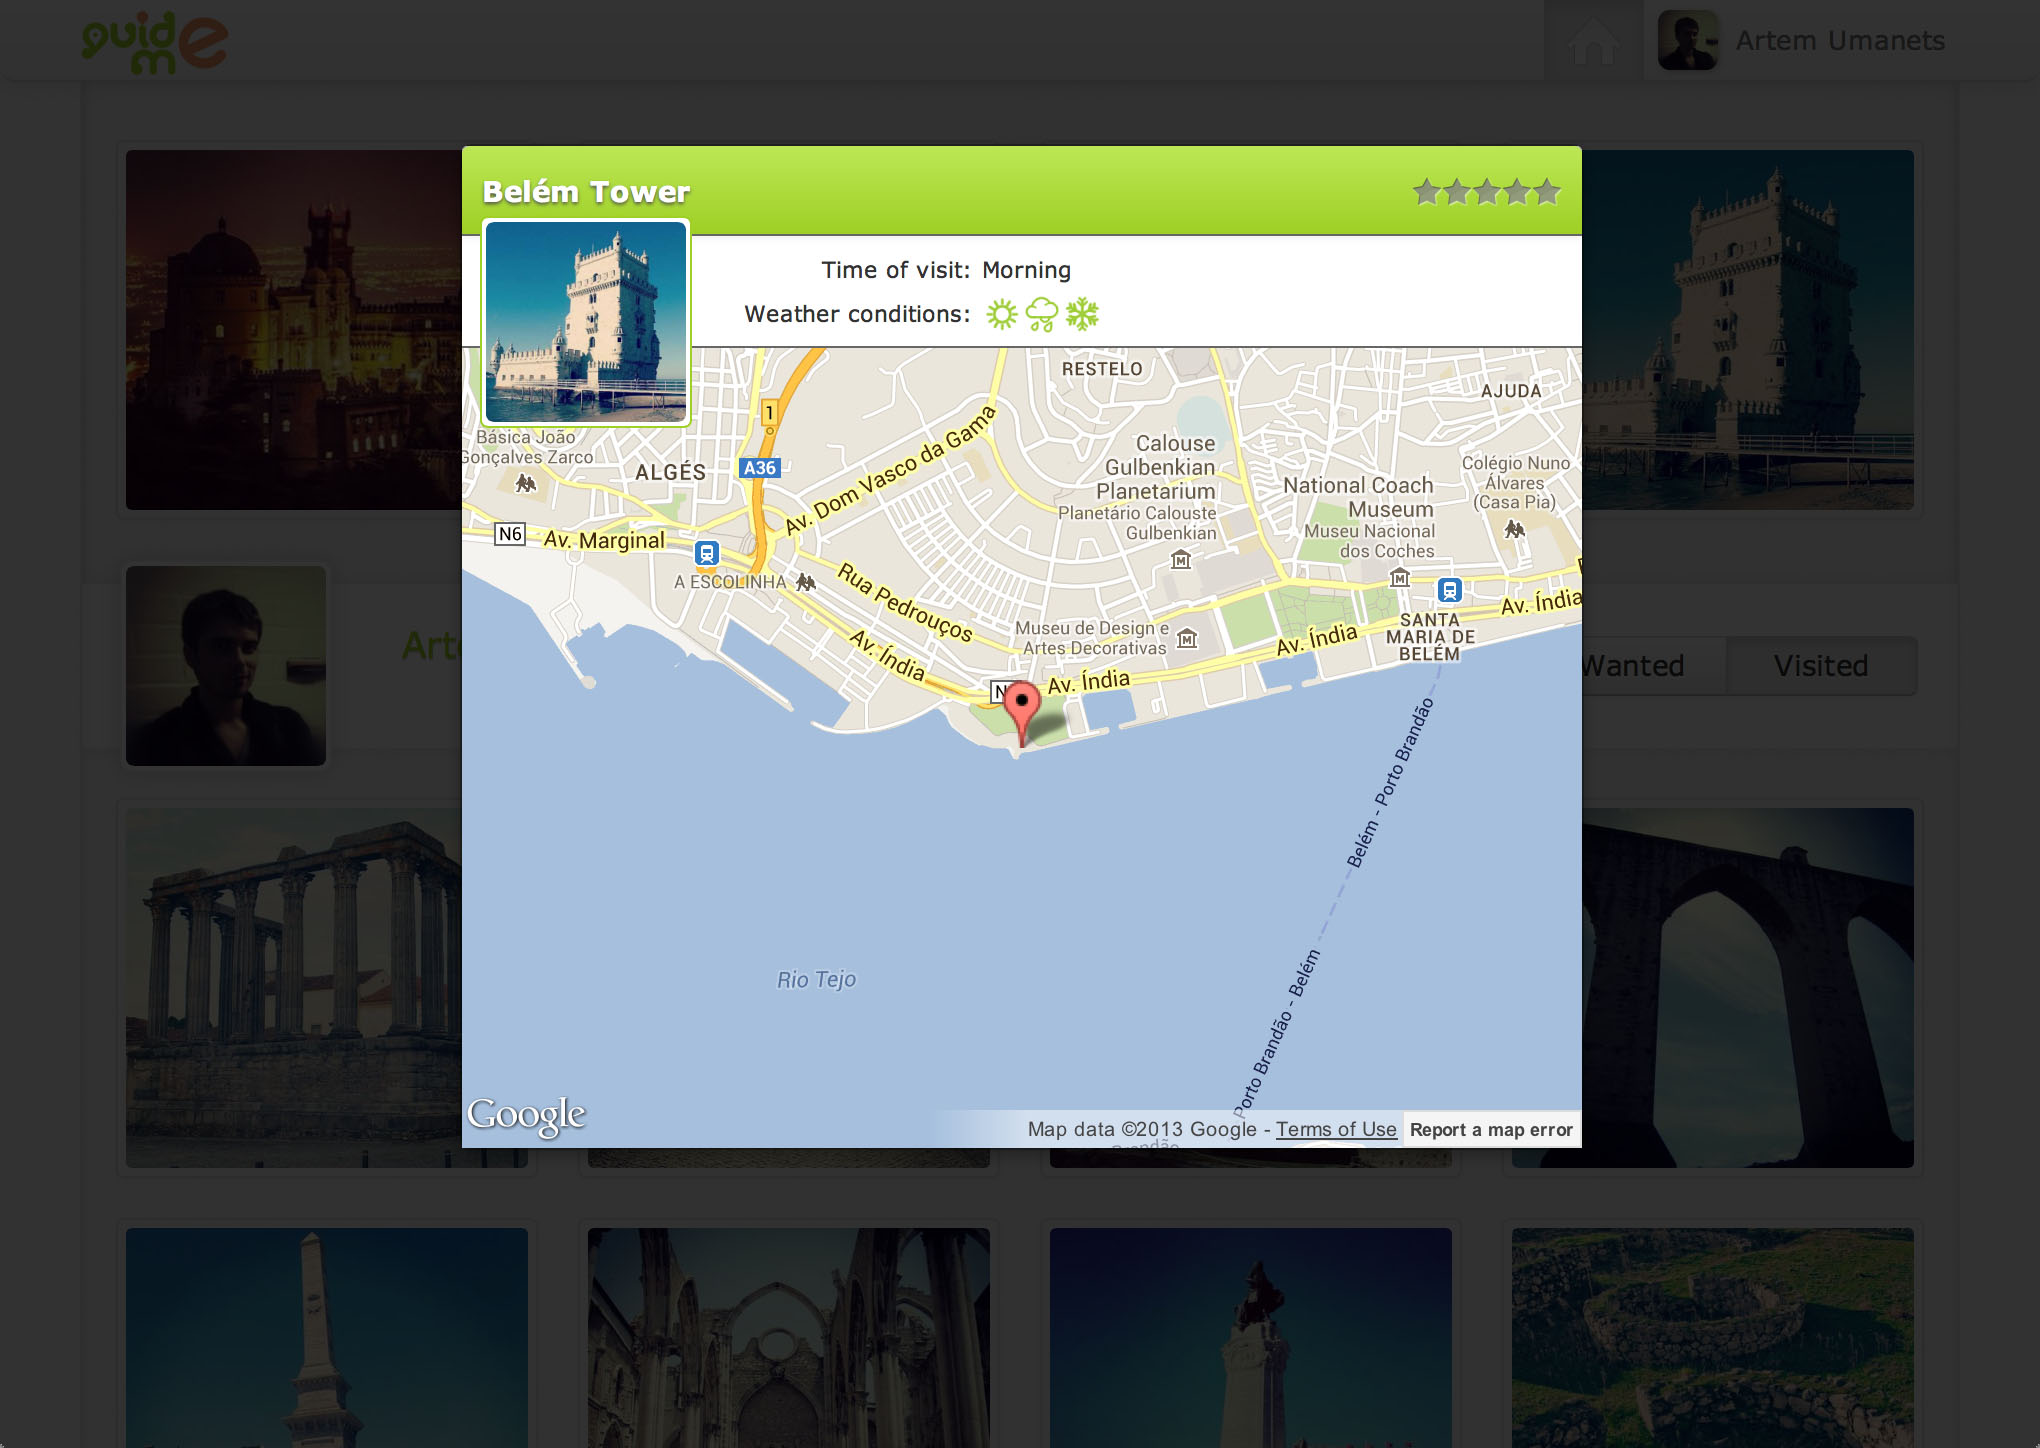
\includegraphics[height=5.2cm]{./images/screenshots/screenshot_web_app_2.jpg}
                \caption{Location details.}
                \label{fig:guidemeWebScreenshotsFina2}
        \end{subfigure}
        \caption{Screenshots of the Web application}
        \label{fig:guideMeWebScreenshotsFull}
\end{figure}
%%%%%%%%%%
%%%%%%%%%%
\subsection{Internationalization Support}
\label{subsec:webAppInternationaization}
The Web application supports localized content using the same mechanism as the \gls{rest}~\gls{api}. The HTTP cookie~\cite{httpCookie} with the language identifier is populated on the first request, and by default it refers to the English language. The action that changes the language overrides the language identifier with a new value which can be changed from either the login or profile page.\\
\\
Some Web operations are implemented in asynchronous mode using the \gls{js} and \gls{ajax} technologies in order to make the user's interaction more intuitive. We have used jQuery~\cite{jquery} library to make the development of the \gls{js} code easier and more readable. The Scala template engine is not able to parse the external \gls{js} files, so a problem with localized messages appeared when it became necessary to show messages to user through \gls{js}. The solution that was found consisted in using the extension for i18n properties for the jQuery library, consist in performing the \gls{ajax} request to the implemented endpoint \verb"/i18n", which returns the content of the appropriate messages file from the \verb"/conf" directory. Then the localized messages can be accessed as follows: \verb"$.i18n.prop(""\verb"MessageKey""\verb")".
%%%%%%%
%%%%%%%
\subsection{REST API Documentation}
\label{subsec:restAPIDcos}
Users with the administrative role can consult the documentation of the \gls{rest}~\gls{api} on their profile page. Each endpoint is described as a separate text file located in the \verb"public/api" directory. The template for the documentation file is shown in Code Listing~\ref{cod:docFileStrcuture}:\\
\begin{lstlisting}[language=Java,caption={Organization of the documentation information.},label={cod:docFileStrcuture}, frame=bt,belowskip=3em]
@->Title:<Title>
@->Description:<Endpoint Description>
@->Method:<HTTP Method>
@->Url:<Endpoint URL>
@->AuthenticationRequired:<Indicates when authentication is required>
@->Permission:<User Permissions>
@->RequiredParameters:
param1[Type] - Description of parameter1
...
@->OptionalParameters:
param2[Type] - Description of parameter2
...
@->CallExampleUrl:<Example of the invocation URL>
@->OutputExample:<Example of the response, usually in JSON format>
\end{lstlisting} 
Each property is separated by \verb"@->" and the first \verb':' separates the property name from its content. The endpoints are obtained by listing all the files from the \verb"public/api" directory. Each of them is mapped into a model that is more easily integrated in the Scala template. An example illustrating the organization of the endpoint documentation is shown in Figure~\ref{fig:exDocEntry}.\\
\begin{figure}[h!]
 \centering
   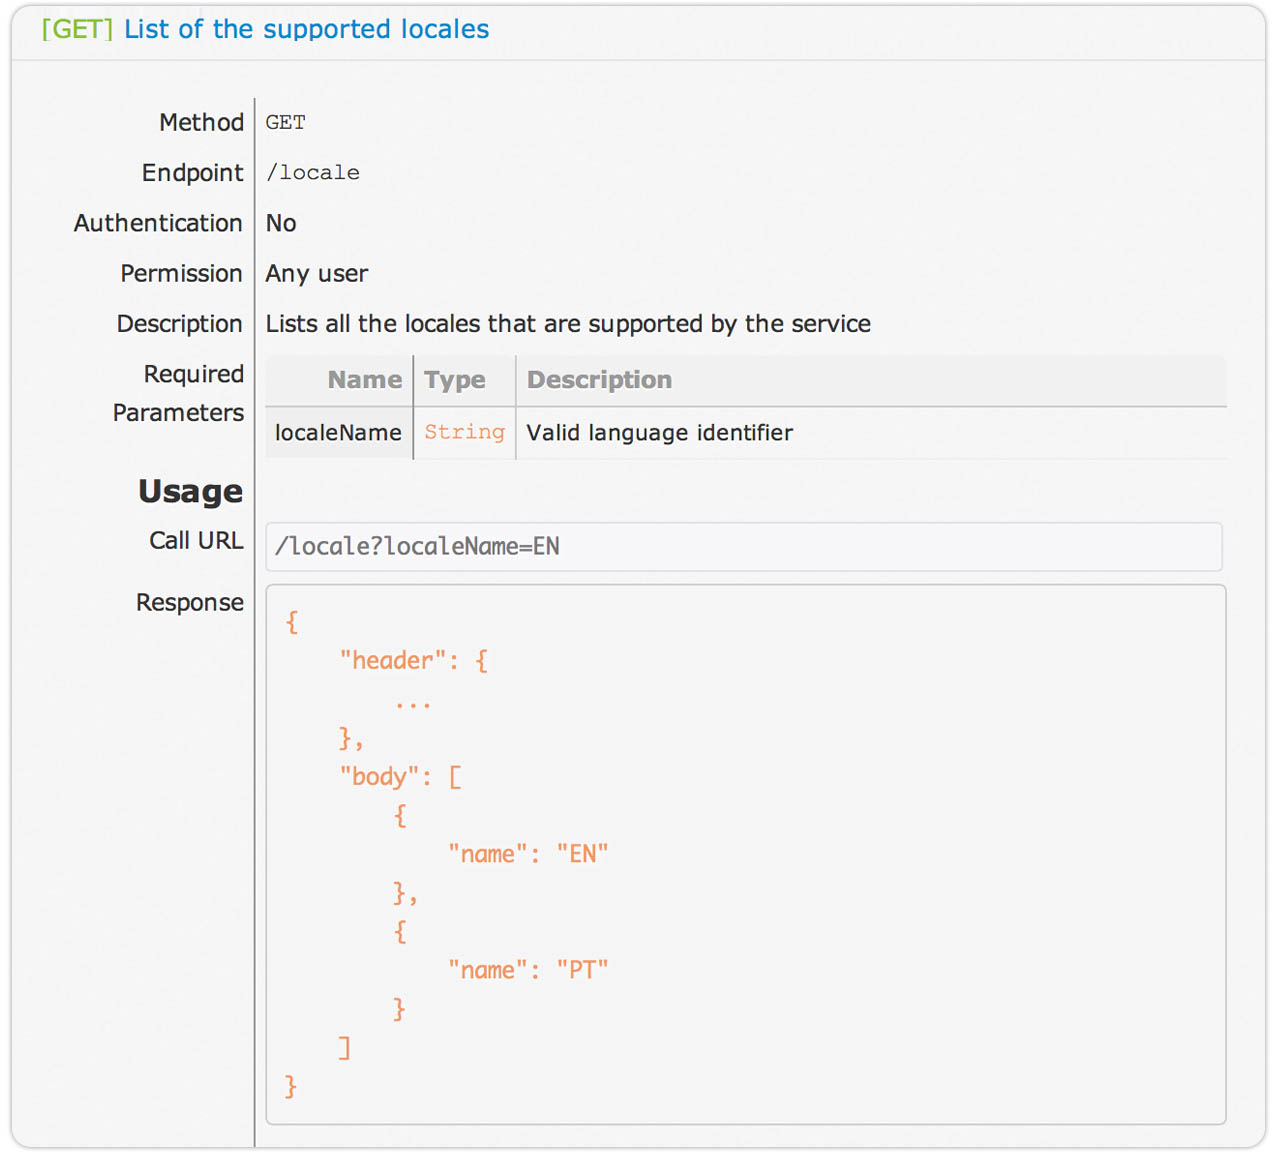
\includegraphics[width=9cm]{./images/examples/example_webapp_documentation.jpg}
   \caption{An example of the documentation entry.}
   \label{fig:exDocEntry}
\end{figure}
\\
The approach for reading and parsing the documentation data is not very efficient. The usage of the database would be more appropriate but we did not want to introduce more databases and complexity to the current project. Improving this part of the project is one of the goals in the future.
%%%%%%%%%%
%%%%%%%%%%
\section{Additional Developments}
\label{sec:additionalImplementation}
In this Section, we describe other developments that were made for this project.
%%%%%
\subsection{Software Testing}
\label{subsec:softwareTesting}
Unitary test methodology is used to check the quality of the code and to facilitate the detection of bugs that may be discovered in the future. Currently, there are around 120 unit test for the \gls{rest} \gls{api} service and 190 unitary test for the Service and Log \gls{dal}. All unitary tests share the same pre-populated database and perform different kinds of operations and queries to ensure that the tested operations perform correct actions.\\
\\
In order to analyse the code coverage, we have used the EclEmma~\cite{codeCoveragEclEmma} plugin for Eclipse IDE. This analysis helped us to improve coverage of the implemented unit tests, lowering the chance of bugs. The implemented unit tests are covering around $90\%$ of the code related to the Service DAL and around $75\%$ of the Log DAL. The uncovered code is mainly related to the entities generated by the Hibernate framework.\\
\\
The iOS application implements 35 unit tests which aim is to perform the remote requests to the~\gls{rest} API. These tests help to detect any unpredictable changes that may emerge in the future.
%%%%%
\subsection{Multi Environment Support}
\label{subsec:multiEnvironmentSupport}
The DAL and~\gls{rest} API components were carefully designed in order to support multiple environments by mean of configuration. At the DAL layer, it is possible to specify different configuration files for testing and production purposes. The same applies to the~\gls{rest} API, which allows to adjust the configurations that vary between test and production environments.

\subsection{REST API Incoherence}
\label{subsec:restAPIIncoherence}
The developed \gls{rest} API invalidates some concepts of the \gls{rest} architecture due to external causes. Usually, the \verb"DELETE HTTP" method is used for resource removal and \verb"UPDATE HTTP" method updates the resource. Some firewalls may block these HTTP verbs, therefore the API was developed in order to use the POST method for creating, updating and removing the resource and GET to consult its information. The type of the operation is indicated as part of the URL request (e.g. the operation to remove the user is implemented as follows: POST \url{http://host/user/delete?id=5} instead of DELETE \url{http://host/user/5}).